\documentclass{vldb}

\usepackage{balance}  % for  \balance command ON LAST PAGE  (only there!)
\usepackage{dsfont,amssymb,amsfonts,enumitem}
\usepackage{graphicx,xcolor,tikz,comment}

\usepackage{subcaption}
	
%pgfplots configuration
\usepackage{pgfplots}
\pgfplotsset{compat=newest}
\pgfplotsset{ table/search path={TexImg/} }

\usepackage{algorithm,algpseudocode}
\renewcommand{\algorithmicrequire}{\textbf{Input:}}
\renewcommand{\algorithmicensure}{\textbf{Output:}}
\usepackage[colorlinks]{hyperref} 

\usepackage{mathtools}
\DeclarePairedDelimiter{\abs}{\lvert}{\rvert} %
\DeclarePairedDelimiter{\brk}{[}{]}
\DeclarePairedDelimiter{\crl}{\{}{\}}
\DeclarePairedDelimiter{\prn}{(}{)}

\newcommand{\citet}{\cite}%CHANGE THIS
\newcommand{\citep}{\cite}


%Useful commands
\newcommand{\E}{\mathbb{E}} 							%expectation
\newcommand{\Var}{\mathbb{V}\textnormal{ar}} 			%variance
\newcommand{\In}[1]{\mathds{1}_{\left\{ #1 \right\}}} 	%indicator
\newcommand{\R}{\mathbb{R}}								%reals
\newcommand{\N}{\mathbb{N}}								%naturals					
\renewcommand{\Pr}{\mathbb{P}}							%probability
\newcommand{\anote}[1]{{\color{red}Alberto: #1}}		%to leave notes
\newcommand{\sbnote}[1]{{\color{blue}Sid: #1}}			\newcommand{\sbedit}[1]{{\color{blue} #1}}			%to leave notes
\newcommand{\todo}[1]{{\color{green}TODO: #1}}		    %to leave notes
\newcommand{\norm}[1]{\lvert\lvert#1\rvert\rvert}		%norm	
\newcommand{\card}[1]{\lvert#1\rvert}					%cardinal of a set
\newcommand{\ceil}[1]{\lceil#1\rceil}					%ceiling function
\newcommand{\Or}{O}

\newcommand{\defeq}{\coloneqq}



%Additional commands
\newcommand{\calP}{\mathcal{P}}							%Set of paths
\newcommand{\calQ}{\mathcal{Q}}							
\newcommand{\Nf}{\mathcal{N}^+}							%forward neighborhood
\newcommand{\Nb}{\mathcal{N}^-}							%reverse neighborhood

\newcommand{\Bf}{B^+}									%forward ball
\newcommand{\Bb}{B^-}									%reverse ball
\newcommand{\Sf}{S^+}
\newcommand{\Sb}{S^-}
\newcommand{\Lf}{L^+}									%forward hub
\newcommand{\Lb}{L^-}									
\newcommand{\dist}{\mbox{dist}}							%distance
\newcommand{\pp}[1]{\langle#1\rangle}					%to denote a path
\newcommand{\PE}{\mathcal{P}^E}							%efficient paths
\newcommand{\PB}{\mathcal{P}^B}							%shortest in G^B
\newcommand{\Pst}{\mathcal{P}_{s,t}}					%all paths s-t
\newcommand{\PS}{\mathcal{P}^*}							%shortest
\newcommand{\Gp}{\tilde G}								%pruned augmented graph
\newcommand{\Ep}{\tilde E}								
\newcommand{\Vp}{\tilde V}			
\newcommand{\hc}{h_c}				
\newcommand{\Lm}{L_{\mathrm{max}}}

\newtheorem{theorem}{Theorem}
\newtheorem{proposition}{Proposition}
\newtheorem{corollary}{Corollary}
\newtheorem{lemma}{Lemma}
\newdef{definition}{Definition}
\newdef{remark}{Remark}

\newenvironment{proofof}[1]{\begin{proof}[{\rm\sc of #1}]}{\end{proof}}

\begin{document}

% ****************** TITLE ****************************************

\title{Computing Constrained Shortest-Paths at Scale}


% ****************** AUTHORS **************************************

\numberofauthors{3} 

\author{
\alignauthor
Alberto Vera\\
\affaddr{Cornell University}\\
\email{aav39@cornell.edu}
% 2nd. author
\alignauthor
Siddhartha Banerjee
\affaddr{Cornell University}\\
\email{sbanerjee@cornell.edu}
% 3rd. author
\alignauthor
Samitha Samaranayake          \\               
\affaddr{Cornell University}\\
\email{samitha@cornell.edu}
}

\maketitle

\begin{abstract}
We study the problem of computing constrained shortest paths at scale, motivated by the needs of modern transportation platforms for travel-time estimates with probabilistic guarantees. 
The use of preprocessing techniques and network augmentation has led to dramatic improvements in the speed and scalability of shortest path (SP) computations.
Our work extends these ideas to CSP queries, via two main contributions: 
\begin{itemize}[nosep,leftmargin=*]
\item We adapt existing preprocessing techniques for fast SP queries (in particular, hub labels) to handle CSP queries; we also extend the \emph{highway-dimension}, a measure of graph structure that enables SP speedup techniques, to an analogous \emph{constrained highway dimension} for CSP queries.
Finally, we show that the two notions can be related under an additional partial witness condition.
\item We develop a practical algorithm for fast CSP queries, combining hub labels with an augmented graph that encodes efficient paths. We evaluate our algorithm on datasets with detailed travel-time information for San Francisco and Luxembourg, and show that our algorithms are orders of magnitude faster compared to existing techniques, and also have small per-node storage requirements, and good preprocessing times even on a single machine. 
\end{itemize}	
\end{abstract}

\section{Introduction}
	%!TEX root = main_vldb.tex


We consider the problem of fast computation of constrained shortest paths in large-scale graphs, using preprocessing and graph augmentation techniques.
The Shortest-path (SP) computation problem is one of the canonical algorithm design problems.
In recent years, however, it has been revolutionized both in terms of academic research as well as real-world applications (cf.~\cite{dimacs09,goldberg_survey} for surveys).
In particular, the use of preprocessing techniques and network augmentation has led to dramatic improvements in the speed and scalability of SP computation in road networks.
These techniques however do not extend to constrained shortest-path (CSP) computations, and our work aims to bridge this gap.


The SP and CSP problems can be summarized as follows: We are given a graph $G$, where each edge has an associated \emph{length} and \emph{cost}. 
Now, given any two nodes $s,t$, the SP problem requires finding an  $s\rightarrow t$ path of minimum length; the CSP problem takes in a further input of a budget $b$, and requires finding a minimum length $s\rightarrow t$ path \emph{which moreover has a total cost less than $b$}.
The two problems, though similar, have very different basic complexity: SP computation admits a polynomial-time algorithm (in particular, the famous Dijkstra's algorithm), while the problem of CSP computation is known to be NP-Hard~\cite{csp_survey}.
That said, a standard dynamic programming approach allows CSP computation in pseudo-polynomial time (in particular, polynomial in the maximum budget), and also admits a natural scaling-based FPTAS (akin to the knapsack FPTAS).


Although there is a rich literature on CSP problems (cf. \cite{csp_survey} for a survey), there is little work on studying ways of using preprocessing and graph augmentation to speed up CSP computation. Our work here aims to address this gap, motivated by the success of similar approaches for SP computation. Moreover, we believe that there is a need for such techniques in several modern applications, as we discuss next. 


\paragraph*{Applications of large-scale CSP computation}

Our interest in CSP computation is motivated primarily by the requirements of transportation platforms like Lyft, Uber, Waze etc., for accurate routing and travel-time estimates.
Fast routing and trip-time estimation, driven by fast SP engines (for example, OSRM~\cite{OSRM}), have provided impetus to the increasing use of mobile maps.
These techniques however do not make full use of available real-time traffic information; in particular, SP queries are unable to incorporate uncertainties in travel times, and hence often give inaccurate trip-time estimates in settings with high traffic uncertainty.


A natural way to incorporate travel-time uncertainty is to compute the shortest path subject to a reliability constraint.
In particular, in many settings, we want \emph{robust} travel time estimates: formally, we require that given $s,t$ and parameters $p,\delta$, a routing algorithm returns an $(s,t)$-path $P$ minimizing $\E[\ell(P)]$, subject to $\Pr[\ell(P)>\E[\ell(P)]+\delta]\leq p$.
Even assuming that travel times on different road segments are independent, computing this exactly for general distributions is expensive due to the need for computing convolutions of distributions. However, for uncorrelated travel-times, we have $\Pr[\sum_eT_e>\E[\sum_eT_e])+\delta]\leq \sum_e\Var(T_e)/\delta^2$ by Chebyshev's inequality; using this, we can replace the robust trip-time estimation problem with the following
\[
\min_{ P\in\calP_{s,t}}\sum_{i\in P}\mu_i \qquad \text{s.t.}\qquad \sum_{i\in P}\sigma^2_i\leq \delta^2p.
\]
This is now a CSP problem. Note that the solution, though not necessarily optimal, always respects the reliability constraint -- this is often more critical for practical applications.


Another natural problem that can be modeled as a CSP is that of finding shortest paths satisfying some \emph{reliability constraint}.
Consider the case where each edge has a probability $q_e$ of triggering a bad event, with resulting penalty $p$ (for example, slowdowns due to accidents).
In this case, we want to minimize the travel time as well as the expected penalty.
In this case, assuming independence, we have the following natural problem
\[
\min_{P\in\calP_{s,t}} \ell(P)+p\Bigl(1-\prod_{e\in P}(1-q_e)\Bigr).
\]
This model is considered in \citet{fareevasion} consider (for routing with fare evasion, where $q_e$ is the probability of encountering an inspector, and $p$ the penalty), where the authors suggest using a CSP formulation, wherein the non-linear objective is replaced by a linear constraint by taking logarithms.

Finally, another class of problems which is related to the CSP is that of routing under \emph{label constraints} \cite{language_csp,rice_csp}, wherein we want shortest routes which satisfy certain properties (for example, those that avoid toll roads). Although different in formulation, the main idea in such problems, as in the CSP, is to use an appropriate augmented graph that converts feasible shortest paths to shortest paths. Our theoretical results extend to these applications as well.

\subsection{Our Contributions}

\noindent There are two natural questions re fast CSP computation:
\begin{enumerate}[nosep,leftmargin=*]
\item How can we use preprocessing and graph augmentation techniques to speed up CSP computation 
\item How can we give preprocessing/storage/query time guarantees for such techniques
\end{enumerate}
The concept of Highway Dimension (HD) \cite{highway2010,highway2013} allows to prove the efficiency of shortest path computations in undirected graphs.
We will see that directed graphs are fundamental for the analysis of constrained paths.
As a first step, we extend the notions of HD to directed graphs.

\sbnote{copied from abstract}
Our work extends these ideas to CSP queries, via two main contributions:  \todo{add references to results here}
\begin{itemize}[nosep,leftmargin=*]
	\item Theoretical contributions: We adapt existing preprocessing techniques for fast SP queries (hub labels and contraction hierarchies) to handle CSP queries. More importantly, we extend the idea of \emph{highway-dimension}, a proposed measure of the complexity of SP speedup techniques, to an analogous \emph{constrained highway dimension} for CSP queries.
	We also show that the two notions can be related under an additional partial witness condition, which we argue is natural for road networks.
	\item Practical contributions: We develop a practical algorithm for fast CSP queries, which combines the hub labels technique for SP computations with an augmented graph that encodes efficient paths for the CSP problem. We evaluate our algorithm on datasets with detailed travel-time information for San Francisco and Luxembourg, and show that our algorithms support query times which are orders of magnitude than existing techniques (without preprocessing), have small per-node storage requirements, and good preprocessing times even on a single machine. 
\end{itemize}	


\subsection{Related work}

Bicriteria with augmented graph and robot applications \cite{alex_bicriteria}

Introduced hub labels\cite{cohen_definition_hl}

Survey on shortest path algorithms \cite{goldberg_survey}

Bounds for hub labels in different classes of graphs. 
Show that there exists a hierarchichal hub label meeting the bound of HD \cite{babenko_hl_complexity}

Shows that the lower bounds of the HL size, given by the HD, is tight for a family of graphs \cite{white_complexity_hd}

Introduce a class of restrictions as label constraints \cite{language_csp}

For a restricted language, it is possible to use CH for the problem \cite{rice_csp}

Skeleton dimension \cite{skeleton}

Survey on CSP \cite{csp_survey}

This objective is closely related to the stochastic on time arrival (SOTA) problem \cite{fan2005arriving}.

SOTA problem with gaussian travel times solved by exhaustive search \cite{nikolova_gaussian}, optimal policy \cite{samaranayake2012speedup}, pre-processing \cite{sabran2014precomputation} anb solved with discretization for directed acyclic graphs \cite{nikolova_discretization}

\section{Preliminaries}
\label{sec:prelim}

\subsection{Basic Setting}
\label{ssec:basic}
%!TEX root = main_vldb.tex

We consider a directed graph $G=(V,E)$ with \emph{length function} $\ell:E\to \N$, and \emph{cost function} $c:E\to \N\cup\{0\}$.
For each node $v$, we denote its in-neighborhood as $\Nb$ and out-neighborhood as $\Nf$; the node degree $\Delta(v) = |\Nf|+|\Nb|$.
Finally, we define the maximum degree $\Delta = \max_v\Delta(v)$.


A (simple) \emph{path} $P$ in $G$ is an acyclic sequence of nodes  $\crl*{u_1u_2u_3\ldots u_k}$ with $(u_i,u_{i+1})\in E$~\footnote{By acyclic, we refer to the fact that $u_i\neq u_j$ for any $i\neq j$ and $u_i,u_j\in P$.}. 
For any source-terminal pair $s,t\in V$, we denote by $\calP_{s,t}$ the set of all paths from $s$ to $t$.

The length $\ell(P)$ is the sum of edge lengths in $P$; by convention, a path with a single node $v$ has length zero.
For $s,t\in V$, the distance from $s$ to $t$, denoted $\dist(s,t)$, is the smallest length among all paths $P$ that start at $s$ and terminate at $t$.
The distance from a node $v$ to a path $P$, denoted $\dist(v,P)$, is measured as the minimum distance from $v$ to a node $w\in P$.
The distance to $v$, $\dist(P,v)$, is defined analogously~\footnote{Note that  $\dist(P,v)$ and  $\dist(v,P)$ need not be the same as the graph is directed.}.
We denote the shortest $(s,t)$-path (if it exists) as $P(s,t)$, and denote the set of all shortest paths in $G$ as $\calP$.



Analogous to length, we define the cost $c(P)$ as the sum of edge costs on path $P$. 
Our goal is to develop a data structure that enables fast computation of \emph{efficient paths}
\begin{definition}
\textbf{(Efficient Paths)} A path $P\in \calP_{s,t}$ is said to be \emph{efficient} if there is no other path $P'\in \calP_{s,t}$ such that $\ell(P')\leq \ell(P)$ and $c(P')\leq c(P)$ with at least one inequality strict.
\end{definition}
We denote the set of all efficient paths as $\PE$, and define the \emph{Pareto frontier} from $s$ to $t$ as $\calP_{s,t}\cap\PE$.
Observe that every subpath of an efficient path is also efficient (if not, we could improve the path by replacing the subpath).


For $r>0$ and $v\in V$, we define the \emph{forward and reverse balls of radius $r$} by $\Bf_r(v)\defeq\{u\in V: \dist(v,u)\leq r\}$ and $\Bb_r(v)\defeq\{u\in V: \dist(u,v)\leq r\}$, and denote $B_r(v)\defeq\Bf_r(v)\cup\Bb_r(v)$.
The graph $G$ is said to have a \emph{doubling dimension} $\alpha$ if, for any node $v$ and any $r>0$, the ball $B_{2r}(v)$ can be covered by at most $\alpha$ balls $B_r(w)$ of radius $r$. 




\subsection{Hitting sets and the highway dimension}
\label{ssec:hddef}
%!TEX root = main_vldb.tex

We now define the notions of hitting sets for path systems, and the highway dimension (HD), which we use to parametrize the performance of our algorithms. The highway dimension was introduced by Abraham et al.~\cite{highway2010,highway2013} for undirected graphs and the shortest-path set system. 
Our presentation closely follows these works.
However, we need to extend the definitions to directed graphs and general path systems for our purposes. 

We define a \emph{path system} $\calQ$ as any collection of paths.
Given a set $C\subseteq V$ and a path $Q$, we say that $C$ \emph{hits} $Q$ if some node in $Q$ belongs to $C$. Moreover, we say that $C$ is a \emph{hitting set for a path system} $\calQ$ if it hits every $Q\in\calQ$.

Hitting sets are useful for compressing path systems. In particular, though a hitting set may be large, the extent to which a path system can be compressed depends on the \emph{local sparsity} of a hitting set with respect to \emph{significant paths} of $\calQ$. 
Following \cite{highway2013}, for any $r>0$, we say a path $Q$ is $r$-significant $\ell(Q)>r$. For a given path-system $\calQ$, we denote $\calQ_r$ as the set of all $r$-significant paths in $\calQ$.
\begin{definition}
\label{def:lshs}
\textbf{(Locally-Sparse Hitting Sets)} Given a path system $\calQ$ and $r>0$, an $(h,r)$ locally-sparse hitting set (or $(h,r)$-LSHS) is a set $C\subseteq V$ with two properties: 
\begin{enumerate}[nosep]
\item Hitting: $C$ is a hitting set for $\calQ_r$.
\item Local sparsity: for every $v\in V$, $\abs*{B_{2r}(v)\cap C}\leq h$.
%$\card{\Bb_{2r}(v)\cap C}\leq h$ and $\card{\Bf_{2r}(v)\cap C}\leq h$.
\end{enumerate}
\end{definition}


The existence of $(h,r)$-LSHS enables the compression of path-system $\calQ$ via the construction of \emph{hub labels} (cf. Section~\ref{ssec:hldef}). However, existence is not sufficient to guarantee efficient computation. 
To circumvent this, Abraham et al.~\cite{highway2013} introduced the notion of the \emph{highway dimension} -- a property of the graph which ensures both existence and efficient computation of LSHS. 

We first need two additional definitions:
for $v\in V, r>0$, we define the \emph{forward and reverse path-neighborhoods} with respect to path-system $\calQ$ as 
\begin{align*}
S_r^+(v,\calQ) &\defeq\crl*{Q\in\calQ_r: \dist(v,Q)\leq 2r}, \\  
S_r^-(v,\calQ) &\defeq\crl*{Q\in\calQ_r: \dist(Q,v)\leq 2r},
\end{align*}
and as before, we have $S_r(v,\calQ) = S_r^+(v,\calQ)\cup S_r^-(v,\calQ)$. Now we can define the highway dimension (HD) of $G$. Essentially, the HD re-orders the sequence of qualifiers in the definition of $(h,r)$-LSHS: it requires the existence of a small hitting set for each individual neighborhood, rather than a single hitting set which is locally sparse. 
\begin{definition}
\label{def:hddef}
\textbf{(Highway Dimension)}
A path-system $\calQ$ has HD $h$ if, for every $r>0$, and for every $v\in V$, there exist sets $H_{v,r}\subseteq V$ such that $\card{H_{v,r}}\leq h$ and $H_{v,r}$ is a hitting set for $S_r^+(v,\calQ)\cup S_r^-(v,\calQ)$.
\end{definition}
The HD was defined in \cite{highway2013} for undirected graphs and the shortest-path system $\calP$. 
The above definition is the natural analog for directed graphs and general set systems (as shorthand, we refer to the HD of $(G,\ell)$ as that of the shortest-path system $\calP$). 
To see that $HD\leq h$ is a more stringent requirement than the existence of an $(h,r)$-LSHS $C$, note that $C\cap B_{2r}(v)$ need not hit all the paths in $S_r(v,\calQ)$. 
However, if $G$ has $HD\leq h$, then this guarantees the existence of a $(h,r)$-LSHS.
\begin{proposition}
If the path system $\calQ$ has HD $h$, then, $\forall\,r>0$, there exists an $(h,r)$-LSHS.
\end{proposition}
This follows directly from Theorem 4.2 in \cite{highway2013}, which showed it for the shortest-path system. More importantly, as we discuss in Section~\ref{sec:preproc}, if $G$ has HD$\leq h$, then this permits efficient computation of locally-spare hitting sets; in particular, for any $r$, a simple greedy algorithm gives an $(h\log n,r)$-LSHS, and a more complex algorithm (which is still poly-time) gives an $(h\log h,r)$-LSHS.


Finally, we note that for pedagogical reasons, Definition~\ref{def:hddef} differs slightly from \cite{highway2013}; in particular, we consider a less restrictive definition of path neighborhoods (albeit for general path systems) that is appropriate for our needs. Consequently the highway dimension as returned by our definition is smaller than that of \cite{highway2013}~\footnote{In particular, unlike \cite{highway2013}, the HD of $G$ as per our definition is not an upper bound to the maximum degree $\Delta$ or the doubling dimension $\alpha$.}.
We discuss the relation between the two definitions in detail in Appendix \ref{app:generalhd}. 



\subsection{Shortest-Paths via Hub Labels}
\label{ssec:hldef}
Arguably the two most successful algorithms for the SP problem are CH and HL.
When a network has small HD, it is possible to obtain efficient structures for both of these algorithms.
We explain here the construction for HL.
For the construction of CH see Section~\ref{sec:ch}.

The HL algorithm is described as follows.
Every node $v$ is assigned two sets of nodes, $\Lf(v)$ and $\Lb(v)$, referred to as forward and backward hubs.
We store $\dist(v,w),\dist(u,v)$ for every $w\in\Lf(v),u\in\Lb(v)$.
The hubs are said to satisfy the cover property if, for any $s\neq t\in V$, $\Lf(s)\cap\Lb(t)$ contains at least one node in $P(s,t)$.
In the case that $t$ is not reachable from $s$, it must be that $\Lf(s)\cap\Lb(t)=\varnothing$.

With the cover property it is trivial to obtain $\dist(s,t)$; we just compare all nodes $w\in\Lf(s)\cap\Lb(t)$ and return the minimum of $\dist(s,w)+\dist(w,t)$.
If the hubs are ordered by ID, we can obtain the distance with a single coordinated sweep in time $\Or(\card{\Lf(s)}+\card{\Lb(t)})$.
Note that the size of the HL bounds both the query time and the storage requirements.
The following result shows how to obtain small HL, the construction of hubs mimics the undirected case.

\begin{theorem}\label{theo:construct_hl}
If $(G,\ell)$ has HD $h$, then we can construct hub labels of size at most $h\log D$.
\end{theorem}
\begin{proof}
The hubs are defined as
\begin{align*}
\Lf(v):&=  \bigcup_{i=1}^{\log D}C_i\cap \Bf_{2^i}(v)\\
\Lb(v):&= \bigcup_{i=1}^{\log D}C_i\cap \Bb_{2^i}(v).
\end{align*}
Since $C_i$ is an $(h,2^{i-1})$-LSHS and we intersect with balls of radii $2\cdot 2^{i-1}$, every set in the union contributes at most $h$ elements and the maximum size is as claimed.

To prove the cover property, we note that, if $t$ is not reachable from $s$, by definition $\Lf(s)\cap\Lb(t)=\varnothing$.
This is because the elements in $\Lf(s)$ are reachable from $s$ and the elements in $\Lb(t)$ reach $t$.

In the case that $P(s,t)$ exists, take $i$ such that $2^{i-1}<\ell(P(s,t))\leq 2^i$.
The path $P(s,t)$ is hit by $C_i$ and any point in the path belongs to both $\Bf_{2^i}(s)$ and $\Bb_{2^i}(t)$.
Such point hitting $P(s,t)$ is then in both hubs, which shows the result.
\end{proof}

\subsubsection{Distance Oracles and Path Computation} \label{sec:path_oracl}
The previous construction is for distance oracles, i.e., they return the length of the SP, but not the path itself.
It is possible to recover the path with additional data; if we double the storage and compute not only the distance to $w\in\Lf(v)$, but also the second node in $P(v,w)$, then it is easy to recover the path.
Each time we run a HL query, at least one node $w\in P(s,t)$, $w\neq s,t$, is returned and we sequentially run queries for the subpaths $P(s,w)$ and $P(w,t)$.
Note that we do need to store this extra information, for example, it could be that $\Lf(s)\cap\Lb(t)=\{s\}$, so the process cannot continue without an additional node.


\section{Scalable CSP Algorithms:\texorpdfstring{\\}{ } Theoretical Guarantees}
%\section{Constrained HD}
\label{sec:chd}
We now turn to the problem of constructing hub labels for constrained shortest-paths queries and, in particular, for computing efficient paths in $G$. 
We want to develop a data-structure that supports fast queries for \emph{efficient paths}. 

In Section \ref{ssec:hldef} we discussed that, if a graph $G$ has HD $\leq h$, we can simultaneously bound, as functions of $h$, the preprocessing time, storage requirements and query time for constructing HL.
This suggests that for the construction of provably efficient HL for the CSP problem, one needs to define an analogous property for the set of \emph{efficient paths}.
\begin{definition}[Constrained Highway Dimension] The constrained highway dimension (CHD) of $(G,\ell,c)$, denoted $h_c$, is the HD of the efficient-path system $\PE$.
\end{definition}
Note that every shortest path is efficient, thus $h_c\geq h$, where $h$ is the HD of $G$ under shortest paths.

We now have two main issues with this definition: first, it is unclear how this can be used to get hub labels, and second, it is unclear how the corresponding hub labels compare with those for shortest-path computations. 
To address this, we first convert efficient paths in $G$ to shortest paths in a larger \emph{augmented graph}. 
In Section \ref{ssec:hlcsp}, we use this to construct hub labels for CSP queries whose storage and query complexity can be bounded as $Bh_c$ (which can be strengthened further to $g(b)h_c$, where $g(b)$ measures the size of the Pareto frontier, cf. Section~\ref{sec:frontier}.). 
Finally, in Section \ref{ssec:hdvschd}, we show that the hub labels for CSP queries can in fact be related to the hub labels for SP queries under an additional natural condition on the efficient paths.

\subsection{Augmented Graph}
\label{ssec:aug}
% !TEX root = main_vldb.tex
\label{sec:augmented}
In order to link the constrained highway dimension to hub labels, we first convert the original graph $G$ (with length and cost functions) into an \emph{augmented graph} $G^B$ with only edge lengths, such that the \emph{efficient paths of $G$ are in bijection with the shortest paths of $G^B$}, i.e. it satisfies
\begin{enumerate}[nosep]
\item All paths starting from a given node are feasible, i.e., they satisfy the budget constraint in $G$.
\item Efficient paths become shortest paths.
\item Inefficient paths are not shortest paths.
\end{enumerate}
We achieve this as follows: Each node in $G^B$ is of the form $\pp{v,b}$, which encodes the information of the remaining budget $b\geq 0$ and location $v\in V$.
A node is connected to neighbors (according to $E$) as long as the remaining budget of that transition is non-negative.
Finally, we create $n$ sink nodes, denoted $v^-$, and connect node $\pp{v,b}$ to $v^-$ with length $1/(b+1)$.
An illustration of the construction is presented in Figure~\ref{fig:augmented}.
The following definition formalizes this. 

\begin{definition}
Given a network $(G,\ell)$ and $B\in\N$, the augmented version $G^B=(V^B,E^B,\ell)$ is defined by
\begin{align*}
V^B &\defeq\crl*{\pp{v,b}: v\in V, b=0,1,\ldots,B}\cup\crl*{v^-:v\in V},\\
E^B &\defeq\crl*{(\pp{v,b},\pp{v',b'}) : vv'\in E, b'=b-c_{vv'}, b'\geq 0}\cup E^{B}_{-},\\
E^{B}_{-} &\defeq \crl*{(\pp{v,b},v^-): v\in V, B\geq b\geq 0}
\end{align*}
and with length function $\ell(\cdot)$,
\begin{align*}
\ell(\pp{v,b},v^-) \defeq \frac{1}{b+1}\;,\;
\ell(\pp{v,b},\pp{v',b'}) \defeq \ell(vv').
\end{align*}
\end{definition}

\begin{figure}
\begin{center}
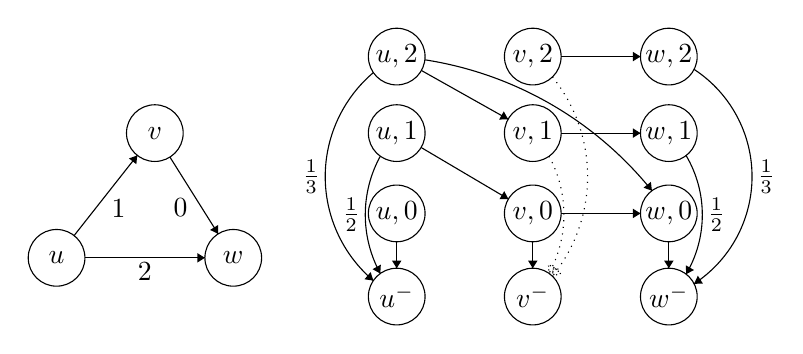
\begin{tikzpicture}[scale=0.12]
\tikzstyle{every node}+=[inner sep=0pt]
\draw [black] (5,-34.3) circle (3);
\draw (5,-34.3) node {$u$};
\draw [black] (15.4,-21.1) circle (3);
\draw (15.4,-21.1) node {$v$};
\draw [black] (23.7,-34.3) circle (3);
\draw (23.7,-34.3) node {$w$};
\draw [black] (41,-13) circle (3);
\draw (41,-13) node {$u,2$};
\draw [black] (41,-21.1) circle (3);
\draw (41,-21.1) node {$u,1$};
\draw [black] (41,-29.6) circle (3);
\draw (41,-29.6) node {$u,0$};
\draw [black] (41,-38.4) circle (3);
\draw (41,-38.4) node {$u^-$};
\draw [black] (55.4,-13) circle (3);
\draw (55.4,-13) node {$v,2$};
\draw [black] (55.4,-21.1) circle (3);
\draw (55.4,-21.1) node {$v,1$};
\draw [black] (55.4,-29.6) circle (3);
\draw (55.4,-29.6) node {$v,0$};
\draw [black] (55.4,-38.4) circle (3);
\draw (55.4,-38.4) node {$v^-$};
\draw [black] (69.8,-13) circle (3);
\draw (69.8,-13) node {$w,2$};
\draw [black] (69.8,-21.1) circle (3);
\draw (69.8,-21.1) node {$w,1$};
\draw [black] (69.8,-29.6) circle (3);
\draw (69.8,-29.6) node {$w,0$};
\draw [black] (69.8,-38.4) circle (3);
\draw (69.8,-38.4) node {$w^-$};
\draw [black] (6.86,-31.94) -- (13.54,-23.46);
\fill [black] (13.54,-23.46) -- (12.66,-23.78) -- (13.44,-24.39);
\draw (10.77,-29.12) node [right] {$1$};
\draw [black] (17,-23.64) -- (22.1,-31.76);
\fill [black] (22.1,-31.76) -- (22.1,-30.82) -- (21.25,-31.35);
\draw (18.92,-29) node [left] {$0$};
\draw [black] (8,-34.3) -- (20.7,-34.3);
\fill [black] (20.7,-34.3) -- (19.9,-33.8) -- (19.9,-34.8);
\draw (14.35,-34.8) node [below] {$2$};
\draw [black] (43.98,-13.342) arc (81.20715:38.87551:38.409);
\fill [black] (68.01,-27.19) -- (67.9,-26.26) -- (67.12,-26.88);
\draw [black] (43.58,-22.62) -- (52.82,-28.08);
\fill [black] (52.82,-28.08) -- (52.38,-27.24) -- (51.87,-28.1);
\draw [black] (58.4,-29.6) -- (66.8,-29.6);
\fill [black] (66.8,-29.6) -- (66,-29.1) -- (66,-30.1);
\draw [black] (43.61,-14.47) -- (52.79,-19.63);
\fill [black] (52.79,-19.63) -- (52.33,-18.8) -- (51.84,-19.67);
\draw [black] (58.4,-21.1) -- (66.8,-21.1);
\fill [black] (66.8,-21.1) -- (66,-20.6) -- (66,-21.6);
\draw [black] (58.4,-13) -- (66.8,-13);
\fill [black] (66.8,-13) -- (66,-12.5) -- (66,-13.5);
\draw [black] (72.471,-14.353) arc (56.79859:-56.79859:13.561);
\fill [black] (72.47,-37.05) -- (73.41,-37.03) -- (72.87,-36.19);
\draw (79.11,-25.7) node [right] {$\frac{1}{3}$};
\draw [black] (71.625,-23.471) arc (30.61438:-30.61438:12.329);
\fill [black] (71.63,-36.03) -- (72.46,-35.59) -- (71.6,-35.09);
\draw (73.84,-29.75) node [right] {$\frac{1}{2}$};
\draw [black] (69.8,-32.6) -- (69.8,-35.4);
\fill [black] (69.8,-35.4) -- (70.3,-34.6) -- (69.3,-34.6);
\draw [black] (38.528,-36.71) arc (-130.31667:-229.68333:14.439);
\fill [black] (38.53,-36.71) -- (38.24,-35.81) -- (37.59,-36.57);
\draw (32.93,-25.7) node [left] {$\frac{1}{3}$};
\draw [black] (39.265,-35.961) arc (-151.22419:-208.77581:12.903);
\fill [black] (39.26,-35.96) -- (39.32,-35.02) -- (38.44,-35.5);
\draw (37.17,-29.75) node [left] {$\frac{1}{2}$};
\draw [black] (41,-32.6) -- (41,-35.4);
\fill [black] (41,-35.4) -- (41.5,-34.6) -- (40.5,-34.6);
\draw [black] (55.4,-32.6) -- (55.4,-35.4);
\fill [black] (55.4,-35.4) -- (55.9,-34.6) -- (54.9,-34.6);
\draw [dotted] (57.481,-15.155) arc (38.87983:-38.87983:16.799);
\draw [densely dotted] (57.48,-36.24) -- (58.37,-35.94) -- (57.59,-35.31) -- cycle;
\draw [dotted] (57.121,-23.549) arc (28.47781:-28.47781:13.004);
\draw [densely dotted] (57.12,-35.95) -- (57.94,-35.49) -- (57.06,-35.01) -- cycle;
\end{tikzpicture}
\end{center}
\caption{Example of a graph augmentation: The original graph $G$ has all paths of unit length, and costs as labeled on the edges. In the augmented graph $G^B$, the labels represent the edge lengths (unlabeled edges have length 1). Note the additional edges from $(w,b)$ to the sink node $w^-$ (and similarly for $u$ and $v$). 
}
\label{fig:augmented}
\end{figure}

Paths in $G^B$ are mapped to paths in $G$ in the intuitive way, by removing the budget labels and sink nodes.
\begin{definition}
Let $P$ be a path in $G^B$.
If $P$ is of the form $\pp{v_1,b_1}\ldots\pp{v_k,b_k}$, then the projection of $P$, denoted $\bar P$, is the path $\bar P\defeq v_1v_2\ldots v_k$.
Analogously, if $P$ is of the form $\pp{v_1,b_1}\ldots\pp{v_k,b_k}v_{k}^-$, then $\bar P\defeq v_1\ldots v_{k}$. 
\end{definition}


\begin{proposition}\label{prop:shorteffic}
A shortest path from source $\pp{s,b}$ to sink node~$t^-$ projects to an efficient path in $G$ solving $\dist(s,t|b)$. 
\end{proposition}
\begin{proof}
Let $P$ be the shortest path from $\pp{s,b}$ to $t^-$, and $\bar P$ its projection.
To reach $t^-$, $P$ must pass through some $\pp{t,b'}$, $b'\geq 0$.
By construction, $P$ consumes $b-b'$ units of resource, hence it is feasible; moreover, $\bar P$ is the shortest among $(s,t)$-paths with cost $b-b'$.
Now assume, by way of contradiction, that $\bar P$ is not efficient.
As $\bar P$ is the shortest using $b-b'$ units of resource, there exists $P'$ such that $\ell(\bar P')\leq \ell(\bar P)$ and $c(\bar P')< c(\bar P)$.
It must be that $P'$ passes through $\pp{t,b''}$, with $b''>b'$.
We argue that, in this case, $P$ would not be a shortest path to $t^-$.
Indeed, 
\[
\ell(P')=\ell(\bar P')+\frac{1}{1+b''}
\leq \ell(\bar P) +\frac{1}{1+b''}
< \ell(\bar P) +\frac{1}{1+b'},
\]
where the last expression is exactly $\ell(P)$.
\end{proof}

We note that the augmented graph is similar to existing techniques for solving CSP via dynamic programming~\cite{alex_bicriteria}.
Such an approach, however, requires that all costs are non-zero, thus the augmented graph is a DAG.
In contrast, we allow edge costs to be zero, and therefore, our augmented graph may contain cycles. 
The following construction will depend on LSHS for the system $\PE$, we call such object an efficient path hitting set (EPHS).

The above result now allows us to relate EPHS of the original graph to LSHS in the augmented graph.
Note that in $G^B$ we are interested only in shortest paths ending in sink nodes (since these project to efficient paths). 
Let $\PB$ be the path system comprising all shortest paths in $G^B$ ending in a sink node.
A hitting set for $\PE$ can be used to obtain a hitting set for $\PB$, but, since the augmented graph has more nodes, the sparsity increases.
 
\begin{proposition}
If the path system $\PE$ admits $(\hc,r)$-EPHS, then $\PB$ admits $(\hc B,r)$-LSHS.
\end{proposition}
\begin{proof}
%We define a set $C^B$ and prove that hits $\PB_r$ and that it is locally sparse.
Given $C$, an $(\hc,r)$-EPHS for $\PE$, define
\begin{equation}\label{eq:hitset}
C^B\defeq \{\pp{v,b}: v\in C, v \text{ hits }\bar P\in\PB_r, c(\bar P)=b\leq B \}.
\end{equation}

By Proposition~\ref{prop:shorteffic}, we know that shortest paths are efficient, hence $C^B$ hits all the desired paths.
Finally, we prove local sparsity.
Take any node $\pp{s,b}$ and observe that
\begin{align*}
\Bf_{2r}(\pp{s,b}) &= \{\pp{t,x}: \exists P\in\Pst, \ell(P)\leq 2r, c(P)=b-x\} \\
&\subseteq \{\pp{t,x}: t\in \Bf_{2r}(s), x\leq b\} .
\end{align*}
We know that $\card{\Bf_{2r}(s)\cap C}\leq \hc$, therefore $\card{\Bf_{2r}(\pp{s,b})\cap C^B}\leq\hc b\leq \hc B$.
A similar argument shows the sparsity for the reverse ball.
\end{proof}

%\begin{remark}
The proof above shows a stronger result:
In Equation~\eqref{eq:hitset} we see that the sparsity around the node $\pp{u,b}$ is $\hc b$.
This is key for our subsequent query time guarantees.
%\end{remark}
%The last result shows how LSHS translate to the augmented graph.
%Since the notion of HD is stronger, it is not always possible to make the analogous between two path systems. Surprisingly, in this case we are able to relate the HD of both path systems.
Moreover, we can also relate the highway dimensions of the path systems $\PE$ and $\PB$ (Note: this does not follow from above, since the HD is a stronger notion than existence of locally-sparse hitting sets).
\begin{proposition}\label{prop:HDaugmented}
If the HD of the system $\PE$ is $h_c$, then the HD of the system $\PB$ is $Bh_c$.
\end{proposition}
\begin{proof}
Fix $r>0$ and $\pp{v,b}\in V^B$ .
Let $H_{v,r}\subseteq V$ be the set hitting $S_r(v,\PE)$ and define $H\defeq H_{v,r}\times\{0,1,\ldots,B\}$.
We show that $H$ hits $\Sf_r(\pp{v,b},\PB)$.

Take $P\in\Sf_r(\pp{v,b},\PB)$.
Since $\dist(\pp{v,b},P)\leq 2r$, it holds $\dist(v,\bar P)\leq 2r$, therefore $\bar P\in \Sf_r(v,\PE)$.
Finally, $H_{v,r}$ hits $\bar P$, thus $H$ hits $P$.
A similar argument shows that $H$ hits $\Sb_r(\pp{v,b},\PB)$.
\end{proof}

In the next section, we discuss how the above augmented graph can be used to construct hub labels for answering CSP queries. 
We note, however, that this technique is primarily a theoretical proof-of-concept, that shows the CHD (and in fact, the HD of $G$ under an additional condition (cf. Section \ref{ssec:hdvschd}) to be a good parametrization for the complexity of HL construction.
In practice (cf. Section \ref{ssec:practical}), we use a similar idea of an augmented graph, but with a construction more amenable for implementation.

\subsection{Hub Labels For CSP}
\label{ssec:hlcsp}
We now describe how to use the augmented graph $G^B$ to get hub labels that allow us to find efficient paths for any query $SP(\pp{s,b},t^-)$.
This is similar to HL construction for shortest-paths (cf. Section \ref{ssec:hldef}).
A subtle difference is that we are only interested in paths ending in a sink node.

Each node $\pp{v,b}$ has a forward hub label $\Lf(\pp{v,b})\subseteq V^B$, and \emph{only sink nodes} $u^-$ have a reverse hub $\Lb(u^-)\subseteq V^B$.
The cover property must be satisfied for every $\pp{s,b}$ and $t^-$.
Finally, if we want to reconstruct the path, we can proceed similarly as in Section~\ref{ssec:hldef}; we can augment the hub labels with the next-hop node, and compute the entire path recursively.

\subsubsection{Query Time and Data Requirements}
Putting things together, we now show how we can construct hub labels for answering CSP queries, such that their preprocessing time and storage is parameterized by the CHD $h_c$.
Note that we use the augmented graph primarily as a theoretical construction.
From a computational point of view, we can obtain the HL using only an EPHS of the original graph.

\begin{theorem}
\label{theo:HLeff}
For graph $(G,\ell,c)$, given a multi-scale EPHS $\crl*{C_i:i=0,1,\ldots,\log D}$, where $C_i$ is an $(h_c,2^{i-1})$-EPHS, we can construct hub labels for answering CSP queries such that, for every $u\in V$ and $b\geq 0$, $\card{L(\pp{u,b})^+}\leq bh_c\log D$ and $\card{L(u^-)^-}\leq Bh_c\log D$. 
\end{theorem}
\begin{proof}
Create $C_i^B$ as in Equation~\eqref{eq:hitset} and define
\begin{align*}
L(\pp{v,b})^+ &\defeq \bigcup_{i=1}^{\log D} C_i^B\cap \Bf_{2^i}(\pp{v,b})\\
L(u^-)^-  &\defeq \bigcup_{i=1}^{\log D} C_i^B\cap \Bb_{2^i}(u^-).
\end{align*}
The cover property is proved similarly as in Proposition~\ref{theo:construct_hl}; we are left to bound the hub size.
For a reverse hub we use that
\begin{align*}
\Bb_{2^i}(t^-) &= \{\pp{s,x}: \exists P\in \Pst, c(P)=x, \ell(P)\leq 2^i\}\\
&\subseteq \Bb_{2^i}(t)\times \{0,1,\ldots,B\}.
\end{align*}
Thus, $\Bb_{2^i}(t^-)\cap C_i^B\leq Bh_c$.
For forward hubs, the size follows from observing that $ \card{C_i^B\cap \Bf_{2^i}(\pp{v,b})}\leq bh_c$.
\end{proof}

This immediately gives us the following corollary for the storage and query time.
\begin{corollary}
Using the HL given by Theorem~\ref{theo:HLeff}, we can implement queries for $s,t,b$ in time $O(b h_c\log D)$.
The total space requirement is $\Or(nB \cdot Bh_c\log D)$.
\end{corollary}

\subsubsection{Preprocessing}
\label{sec:preproc}
\anote{maybe not a subsection of CSP? it applies to any path system (e.g. shortest paths)}
It was shown in \cite{highway2013} that the set system of shortest paths has VC-dimension of $2$.
More formally, paths $v_1v_2\ldots v_k$ are mapped to sets $\{v_1,\ldots,v_k\}$ and this new set system has small VC-dimension.
Observe that, if $G$ is undirected, then each subset represents exactly two paths, namely the $(s,t)$-path and the $(t,s)$-path.
Therefore, a hitting set for the set system corresponds to a hitting set for $\calP$.

Recall that we assume uniqueness of shortest paths.
It is easy to see that the VC-dimension of the previous set system is 2.
Indeed, a path $abc$ is mapped to $\{a,b,c\}$ and the element $\{a,c\}$ would never form a part of the system; the shortest path between $a$ and $c$ must pass through $b$, therefore $\{a,b,c\}$ cannot be shattered.

In directed graphs the same relation can still be made, but the VC-dimension would not be small.
For example, the directed graph can contain the shortest paths $abc$ and $ca$, mapping to sets $\{a,b,c\}$ and $\{c,a\}$, breaking the previous argument.

To overcome this, we now think of paths as sequences of edges.
The ground set for the set system is $E$, instead of $V$ and a path $e_1e_2\ldots e_k$ is mapped to $\{e_1,e_2,\ldots,e_k\}$.
Note that each $\{e_1,e_2,\ldots,e_k\}$ corresponds uniquely to one path.
Recall that in a system $\calQ$ the cycles are not allowed.
We denote $\pi(Q)$ the set of edges in a path $Q$.

\begin{proposition}
Given a system $\calQ$, the corresponding set system $(E,\{\pi(Q):Q\in\calQ\})$ has VC-dimension 2.
\end{proposition}

We now stablish how to obtain polynomial time preprocessing.
Specifically, the algorithms we use are based on the existence of $(h,2^i)$-LSHS.
Assuming a system has HD $h$, we can obtain an approximation of these set, where the sparsity increases by the maximum degree $\Delta$.
The proof can be found in Section~\ref{sec:proofs}.

\begin{proposition}\label{prop:poly_lshs}
If a system $\calQ$ has HD $h$, for some $h'=\Or(h\Delta\log(h\Delta))$ there exists a polynomial time algorithm to obtain a $(h',r)$-LSHS.	
\end{proposition}


\subsubsection{Using the size of the Pareto Frontier}
The linear dependence on $B$ in the bound on HL sizes (cf. \cref{theo:HLeff}) is somewhat weak. 
Essentially, this corresponds to a worst-case setting where the efficient paths between any pair of nodes is different for each budget level. 
In most practical settings, changing the budget does not change the paths too much, and ideally the hub label sizes should reflect this fact. 
This is achieved via a more careful construction of hub labels, resulting in the following bound. 
\begin{theorem}\label{thm:markedhubs}
Let $(G,\ell,c)$ as in \cref{theo:HLeff} and $g:\N\to \N$ be such that, for every $s,t\in V$, $b\in \N$, $\abs{\crl{P\in\Pst^E: c(P)\leq b}} \leq g(b)$.
Then, we can construct hub labels of size $O(g(B)h_c\log D)$, and answer queries with budget $b$ in time $O(g(b)h_c\log D)$.
\end{theorem}

Note that there always exists such a function $g$ and the worst case is $g(b)=b$.
The proof depends on a different technique for constructing HL.
The main idea is to sort the efficient paths for each source node $s$ by cost, and then carefully mark nodes when they are added to forward HL; these marked nodes are then used to construct the reverse HL.
For brevity, the complete algorithmic details and proof are deferred to \cite{TechReport}.

\subsection{Comparing HD and CHD}
\label{ssec:hdvschd}
% !TEX root = main_vldb.tex
The above sections thus show that we can construct hub labels for solving CSP whose preprocessing time, storage and query time can all be parameterized in terms of the constrained highway dimension $h_c$. 
This however still does not give a sense of how much worse the hub labels for the CSP problem can be in comparison with those for finding shortest paths. 
We now try to understand this question.

Comparing the size of the \emph{optimal} hub labels for SP and CSP is infeasible as even finding the optimal hub labels for SP is NP-hard~\cite{babenko_hl_complexity}. However, since we can parametrize the complexity of HL construction for SP in terms of the HD, a natural question is whether graphs with small HD also have a small CHD. Note that the answer to this depends on both the graph and the costs; we now show that in general, the CHD (and in fact, the sparsity of any EPHS) can be \emph{arbitrarily worse} than the HD. 
\begin{proposition}
There are networks with HD $1$ where the CHD, and also the sparsity of any EPHS, is $n$.
\end{proposition}

\begin{figure}
\begin{center}
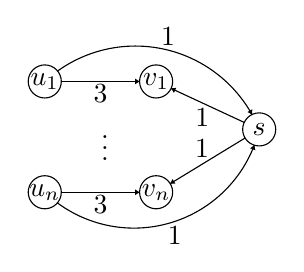
\begin{tikzpicture}[scale=0.07]
\tikzstyle{every node}+=[inner sep=0pt]
\draw [black] (18.5,-12.8) circle (3);
\draw (18.5,-12.8) node {$u_1$};
\draw [black] (38.7,-12.8) circle (3);
\draw (38.7,-12.8) node {$v_1$};
\draw [black] (18.5,-32.9) circle (3);
\draw (18.5,-32.9) node {$u_n$};
\draw [black] (38.7,-32.9) circle (3);
\draw (38.7,-32.9) node {$v_n$};
\draw (29.4,-23.4) node {$\vdots$} ;
\draw [black] (57.4,-21.5) circle (3);
\draw (57.4,-21.5) node {$s$};
\draw [black] (21.5,-12.8) -- (35.7,-12.8);
\fill [black] (35.7,-12.8) -- (34.9,-12.3) -- (34.9,-13.3);
\draw (28.6,-13.3) node [below] {$3$};
\draw [black] (21.5,-32.9) -- (35.7,-32.9);
\fill [black] (35.7,-32.9) -- (34.9,-32.4) -- (34.9,-33.4);
\draw (28.6,-33.4) node [below] {$3$};
\draw [black] (20.825,-10.907) arc (125.59934:29.18714:24.243);
\fill [black] (56.1,-18.8) -- (56.15,-17.85) -- (55.28,-18.34);
\draw (40.87,-6.38) node [above] {$1$};
\draw [black] (56.513,-24.364) arc (-20.88164:-126.45095:23.371);
\fill [black] (56.51,-24.36) -- (55.76,-24.93) -- (56.7,-25.29);
\draw (42.07,-39.01) node [below] {$1$};
\draw [black] (54.84,-23.06) -- (41.26,-31.34);
\fill [black] (41.26,-31.34) -- (42.2,-31.35) -- (41.68,-30.5);
\draw (47.05,-26.7) node [above] {$1$};
\draw [black] (54.68,-20.23) -- (41.42,-14.07);
\fill [black] (41.42,-14.07) -- (41.93,-14.86) -- (42.36,-13.95);
\draw (47.07,-17.66) node [below] {$1$};
\end{tikzpicture}
\end{center}
\caption{Graph with small HD but large CHD: The graph comprises $2n+1$ nodes, with the edge labels representing the lengths. Note that the shortest paths in the graph are of the form $sv_i$, $u_is$ and $u_isv_j$ (for all combinations $i,j$). Thus, the HD is $1$ as $H_{v,r}=\crl{s}$ is a hitting set for all these paths. On the other hand, if we have costs such that $c(u_iv_i)=0\,\forall\,i$, while all other edges have cost $1$; then we have $n$ parallel efficient paths $u_iv_i$, which must all be hit by any EPHS.}
\label{fig:big_chd}
\end{figure}

\begin{proof}
Consider the directed graph $G$ defined in Figure~\ref{fig:big_chd}.
%, which comprises $2n$ nodes $u_i,v_i$ and a special node $s$.
%Every $u_i$ has two outgoing edges, one to $v_i$ with length $3$ and one to $s$ with length $1$.
%Finally, $s$ has $n$ outgoing edges, one to every $v_i$ with length $1$.
%Let us first determine the HD of $G$.
%There are $3n$ shortest paths, namely $sv_i$ and $u_isv_i$ for different $i$.
It is easy to see that $H_{v,r}=\crl{s}$ is a shortest-path hitting set for every $r>0$ and $v\in V(G)$; hence the HD is $1$.
On the other hand, suppose the costs are such that $c(u_iv_i)=0$ for every $i$, while all other costs are set to $1$.
Note that the $1$-significant efficent paths intersecting the ball $B_s(2)$ are $u_iv_i$, which are all disjoint.
Therefore, the hitting set $H_{s,1}$ must contain at least $n$ elements. Moreover, the same argument shows that the sparsity of the best LSHS for $\PS$ is $1$, whereas the sparsity of \emph{any} EPHS is also lower bounded by $n$.
\end{proof}

\begin{remark}
One criticism of the graph in Figure~\ref{fig:big_chd} is that it has a maximum degree of $n$; the result however continues to hold even for bounded degree graphs.
In Appendix~\ref{app:generalhd}, where we discuss alternate notions of HD, we give a more involved example with bounded degrees that exhibits the same separation between HD and CHD for even stronger notions of HD.
\end{remark}

Intuitively, the separation between HD and CHD (or more particularly, the hub labels for computing SPs and CSPs) occurs due to the fact that for arbitrary graphs and cost functions, the shortest and efficient paths may be completely unrelated. 
For real-world networks, however, this appears unlikely -- in particular, intuition suggests that efficient paths largely comprise of segments which are in fact shortest-paths in their own right. This notion can be formalized via the following notion of a \emph{partial witness} 
\begin{definition}
Let $\beta\geq 0$.
We say that a path system $\calQ'$ is a $\beta$-witness of the path system $\calQ$ if, for every $Q\in\calQ$, there exists some $Q'\in\calQ'$ such that $Q'\subseteq Q$ and $\ell(Q')\geq 2^{-\beta}\ell(Q)$.
\end{definition}
Given this definition, we can now ask if the hub labels for computing SPs and CSPs can be related in settings where the shortest-path set system $\PS$ is a partial witness for the efficient path system $\PE$. At an intuitive level, the partial witness property says that efficient and shortest paths are not completely different, i.e., if $Q$ is efficient, a fraction $2^{-\beta}$ of $Q$ is a shortest path.
As a consequence, a node hitting numerous paths in $\PS$, should also hit many paths in $\PE$.
%The bad examples in Proposition~\ref{prop:treelike} exploit networks that do not have partial witnesses.
Note also that asking for the witness property to hold for all lengths is too extreme, as this essentially requires that all single-hop paths with 0 costs are shortest paths; thus, we really want this property only for `long-enough' paths. 


We now show that if costs are such that the graph indeed has the partial witness property (for long-enough paths) for some $\beta$, then we can relate the HL sizes for the two problems in terms of $\beta$ and the doubling dimension $\alpha$. Note that the doubling dimension depends on $G$ and $\ell$; the partial witness property depends on the interplay between $G$, $c$ and $\ell$.
\begin{theorem}\label{theo:witness_doubling}
Assume that $G$ is $\alpha$-doubling and $\PS$ is a $\beta$-witness for $\PE_r$ for every $r\geq \frac{\log(\alpha^\beta h)}{2\log\Delta}$. 
Then, given an $(h,r)$-LSHS for any $r>0$, we can construct (in polynomial time) an $(\alpha^{\beta} h,r)$-EPHS for $(G,\ell,c)$. 
\end{theorem}

\begin{proof}
For any $r$, we need to construct a hitting set $C^E$ for $\PE_r$.
Assume first $r\geq \frac{\log(\alpha^\beta h)}{2\log\Delta}$.
Take $C$ as the hitting set for $\PS_{2^{-\beta}r}$, which is guaranteed to be sparse with respect to balls of radius $2^{-\beta+1}r$.
Define the desired set by
\[
C^E\defeq\{v\in C: v \text{ is in some $r$-efficient path} \}.
\]

Since $\PS$ is a $2^{-\beta}$-witness for $\PE_r$, $C^E$ is indeed a hitting set for $\PE_r$.
We are only left to prove the sparsity.
Take some $u\in V$, by doubling dimension we can cover $\Bf_{2r}(u)$ by at most $\alpha^\beta$ balls of radius $2^{-\beta+1}r$.
Each of these balls contains at most $h$ elements of $C$, therefore the sparsity is as claimed.
The argument for reverse balls is identical.

Now we analyse the case $r< \frac{\log(\alpha^\beta h)}{2\log\Delta}$.
It is no longer true that the efficient paths are witnessed, but now the neigborhoods are small.
Take $C=V$ as the EPHS.
Clearly $C$ hits all the paths and the local sparsity is at most the size of the ball.
Using our assumption on $r$ and the fact that the lengths are integers, it follows that $\card{B_{2r}(v)}\leq\Delta^{2r}\leq\alpha^\beta h$. 
\end{proof}
\begin{remark}
The existence of a $\beta$-witness is not enough to bound the CHD. Nevertheless, as we discuss in Section~\ref{ssec:hldef}, the existence of $(h,r)$-LSHS already allows the construction of HL. Moreover, the above argument does indeed give a bound for a weaker definition of the highway dimension~\cite{highway2010}.
\end{remark}
\begin{remark}
We state the above result in terms of $\alpha, \Delta$ and $h$, in order to make it more transparent. The three quantities are however somewhat related -- in particular, it can be shown that $\alpha\leq 2h\Delta$ (cf.~\cite{skeleton}).
\end{remark}

We finish by observing that the $\beta$-witness property can be relaxed further if we assume something about neighborhoods' growth rate.
We used the crude bound $\card{B_r(u)}\leq \Delta^r$, but some networks exhibit a much different behaviour.
For example, a grid satisfies  $\card{B_r(u)}=\Or(r^2)$, so the bound we used could have an exponential gap.
This implies that we need a witness only for very long paths.

\begin{corollary}
Let $f$ be a function such that, for every $u\in V, r\geq 0$, $\card{B_r(u)}\leq f(r)$ .
Then, assuming only that $\PE_r$ is $\beta$-witnessed for $r\geq f^{-1}(\alpha^\beta h)$,we can get the same guarantee as in Theorem~\ref{theo:witness_doubling}.
\end{corollary}


\section{Scalable CSP Algorithms: \texorpdfstring{\\}{ } Practical Implementation}
\label{sec:numeric}
Our theoretical results in the preceding sections suggest that using hub labels for CSP queries should perform well in road networks, as these are known to have low highway dimension, and potentially also satisfy the (average) partial witness property. The theoretical constructions for hub labels, however, are not directly suitable for large networks, and need significant modifications. We now describe how our techniques can be adapted to give practical hub label constructions, and discuss experimental results for two real world networks using these methods. 
\subsection{Practical CSP Algorithms} 
\label{ssec:practical}

We start by defining a more scalable construction of $G^B$.
The augmented graph $G^B$ defined in \cref{ssec:aug} is not a minimal representation as it may contain a lot of redundant information.
For example, the same efficient path $uv$ can be repeated many times in the form $\pp{u,1}\pp{v,0}$, $\pp{u,2}\pp{v,1}$ and so on.
By encoding this information more efficiently, we get considerable improvements both in query time and in data storage.

We construct our \emph{pruned} augmented graph $\Gp^B$ as follows:
As before, nodes are pairs $\pp{v,b}$, but now we add an edge $\pp{v,b}\pp{v',b'}$ only if it is essential for some efficient path, i.e., removing said edge impacts correctness.
If we let $\Pst^E$ be the set of all efficient paths from $s$ to $t$, we take every $P\in \Pst^E$ with cost $b\leq B$ and trace it in the augmented graph such that it terminates at $\pp{t,0}$.

\begin{definition}\label[definition]{def:pruned_aug_graph}
The pruned augmented graph is defined by $\Gp^B=(\Vp^B,\Ep^B)$, where
\begin{align*}
\Vp^B &:=\crl{\pp{v,b}: v\in V, b=0,1,\ldots,B},\\
\Ep^B &:=\crl{\pp{v,b}\pp{u,x} : \exists s,t\in V, P\in\PE_{s,t}, c(P)\leq B, vu\in P, b=c(P[v,t]), x=c(P[u,t]) }.
\end{align*}
In $\Gp^B$ all the lengths are preserved.
\end{definition}
Note that in $\Gp^B$ there are no sink nodes, hence it has at least $n$ nodes and $nB$ arcs fewer compared to $G^B$.
In the worst case, those $nB$ arcs are the only gain by doing this process.
Nevertheless, in our experiments $\Gp^B$ is up to 60\% smaller than $G^B$.
Observe that, by running Dijkstra in $G^B$, $\Gp^B$ can be computed in time $\Or(n^2B\log(nB))$.

\subsubsection{HD of the pruned augmented graph}

A shortest path in $\Gp$ does not necessarily project to an efficient path, even if the path ends in a node of the form $\pp{t,0}$.
In contrast, if $P$ projects to an efficient path, then necessarily $P$ is shortest. 
To bound the HD, the correct system to study is
\[
\tilde\PB:=\crl{P: P\text{ ends in a node }\pp{t,0}, \bar P\in \PE, c(\bar P)\leq B }.
\]
The following result shows how the HD of this system relates to that of $\PE$.
We omit the proof since it is identical as the one in Proposition~\ref{prop:HDaugmented}.
\begin{proposition}
Given CHD $h_c$, the HD of $\tilde\PB$ is $Bh_c$.
\end{proposition}

\subsubsection{Types of queries}

We test our algorithms with two different tasks.
Recall that our preprocessing is done for some fixed maximum budget $B$.
The first task we consider is a \emph{frontier query}, wherein given $s$ and $t$, we return the lengths of all efficient paths with costs $b=0,1,\ldots,B$.
The second we call a \emph{specific query}, we return $\dist(s,t|b)$ for given $s,t,b$ (i.e., a single efficient path).

Note that the pruned augmented graph $\Gp^B$ is designed for frontier queries.
To see this, fix the terminal $\pp{t,0}$.
As we ask for the shortest path from $\pp{s,B},\pp{s,B-1},\ldots,\pp{s,0}$ we are guaranteed to recover the entire frontier.
On the other hand, it may be that the shortest path between $\pp{s,b}$ and $\pp{t,0}$ does not correspond to $\dist(s,t|b)$.
This occurs when $b$ is not a tight budget and the efficient path requires less.

To answer specific queries, we modify $\Gp^B$ by adding extra edges.
For every $v\in V(G)$ and $b=1,2,\ldots,B$, we include the edge $\pp{v,b}\pp{v,b-1}$ with length $0$.
A simple argument shows that with the added edges, the shortest path between $\pp{s,b}$ and $\pp{t,0}$ has length $\dist(s,t|b)$.

\subsubsection{HL construction via Contraction Hierarchies}

We use some techniques described in \cite{hubimplem} combined with an approach tailored for augmented graphs.
The CH algorithm takes as input any ranking (i.e., permutation) of the nodes, and proceeds by removing nodes from the lowest rank first.
Whenever a node is removed, we add new edges, called shortcuts, if needed to preserve the shortest paths.
Once we have a graph with shortcuts, a CH search is a special variant of Dijkstra where only higher rank nodes are explored, i.e., we never take an edge $uv$ if rank$(u)>\text{rank}(v)$. 
The main idea in our construction is to choose an appropriate ranking, and then define the forward hubs of $v$ as the nodes visited during a contraction-based forward search starting at $v$.
The reverse hubs are defined analogously.
These are valid hubs, since the highest rank node in a path is guaranteed to be in both hubs.

The choice of the ranking function is crucial.
For our experiments, we ranked nodes in $G$ by running a greedy approximate SP cover, selecting the highest rank node as the one covering most uncovered paths in $\PS$ and continuing greedily. 
Specifically, start with a cover $C=\varnothing$ and compute the set of all shortest paths $\PS$.
Take a node $v\notin C$ hitting most paths in $\PS$, then remove all those paths from $\PS$, add $v$ to $C$ and iterate.
The rank is defined as $n$ for the first node added to $C$, $n-1$ for the second and so on.
To implement the SP cover we follow the algorithm in \cite{hubimplem}.
A practical hurdle in such an approach is that to compute a shortest path cover, a direct approach requires storing all the shortest paths in memory, which, in most mapping applications, is infeasible.
To circumvent this, we approximate the shortest-path cover by computing only $k<<n$ shortest-path trees and covering these greedily.
We use an off-the-shelf clustering method to obtain $k$ cluster centers, from which we compute the shortest paths. 
As shown in Figure~\ref{fig:clusters}, the clustering approach provides a very good approximation of the hubs with even a small $k$.
We stress that this is just an easy way to get a ranking; more sophisticated heuristics that decide on-line the next node to contract usually work well in practice \cite{goldberg_survey,rice_csp}.
Using another contraction scheme may expedite our algorithms and reduce the hub size.


Depending on the size of our instance, and the specific queries, we work with either the augmented graph $G^B$ or the pruned augmented graph $\Gp^B$.
Even though $\Gp^B$ takes time to compute, it can speed up the overall process and yield considerably better hubs. 
Given a ranking for nodes in $G$, we contract $\Gp^B$ as follows.
Say that $V$ is ordered according to the ranking, so node~$1$ is the least important and $n$ the most important.
In $\Gp^B$, we first contract the nodes $\pp{1,b}$ for $b=B,\ldots,0$, then the nodes $\pp{2,b}$ and so on till the nodes $\pp{n,b}$ are the last to contract. 
Finally, when contracting a node $v$, if $u$ is a predecessor and $w$ a successor of $v$, we add the short-cut $uw$ only if, by removing $v$, the distance from $u$ to $w$ is altered, and the new shortest path from $u$ to $w$ is efficient.
We can go even further; the short-cut $uw$ is unnecessary if the shortest path is not efficient, even if the distance changes.

To obtain better hubs we prune the results obtained by CH searches.
If $w$ is in the forward search of $v$ with distance $d$, it might be that $\dist(v,w)<d$, this occurs because the search goes only to higher rank nodes and the discovered path is missing some node.
When $\dist(v,w)<d$, we can safely remove $w$ from the hub of $v$, since the highest ranked node in a shortest path will have the correct distance.
For frontier queries, we can also prune away a node $w$ if the $(v,w)$-path has a surplus of budget.
The entire process can be summarized in the following steps.

\begin{table*}

\begin{adjustbox}{max width=\textwidth,keepaspectratio}
\begin{tabular}{| l | p{1cm} | p{1cm} | p{1cm} | p{1.2cm} | p{1.2cm} | }
\hline
	B & Prepro [m] & Avg F Size & Avg B Size & Query Dij [ms] & Query HL [ms] \\ \hline \hline
	0 & 1 & 23 & 22 & 10.71 & 0.005 \\ \hline
5-f  & 5  & 16 & 28 & 80.10  & 0.02 \\
5-s  & 5  & 57 & 28 & 31.75  & 0.01 \\ \hline
10-f & 9  & 9 & 28 & 168.11 & 0.03 \\
10-s & 10 & 68 & 28 & 56.19  & 0.01 \\ \hline
15-f & 12 & 6 & 28 & 237.64 & 0.03 \\
15-s & 16 & 73 & 28 & 77.59  & 0.01 \\ \hline
20-f & 17 & 5 & 28 & 342.47 & 0.03 \\
20-s & 20 & 77 & 28 & 100.26 & 0.01 \\ \hline
25-f & 22 & 4 & 28 & 460.95 & 0.03 \\
25-s & 25 & 80 & 28 & 126.52 & 0.01 \\ \hline
30-f & 26 & 3 & 28 & 569.13 & 0.03 \\
30-s & 31 & 84 & 28 & 152.75 & 0.01 \\ \hline
\end{tabular}%
\quad
\begin{tabular}{ | l | p{1cm} | p{1cm} | p{1cm} | p{1.2cm} | p{1.2cm} |}
\hline
	B & Prepro  [m] & Avg F Size & Avg B Size & Query Dij [ms] & Query HL [ms] \\ \hline \hline
	0 & 6 & 18 & 18 & 16.35 & 0.004 \\ \hline
5-f  & 1  & 18.0 & 18.0 & 175.04  & 0.02 \\
5-s  & 21 & 42.9 & 18.7 & 72.03   & 0.01 \\ \hline
10-f & 2  & 18.0 & 18.0 & 361.15  & 0.04 \\
10-s & 35 & 49.3 & 18.7 & 102.52  & 0.01 \\ \hline
15-f & 3  & 18.0 & 18.0 & 577.89  & 0.06 \\
15-s & 46 & 53.3 & 18.7 & 140.80  & 0.01 \\ \hline
20-f & 4  & 18.0 & 18.0 & 821.94  & 0.07 \\
20-s & 60 & 56.5 & 18.7 & 183.11  & 0.01 \\ \hline
25-f & 5  & 18.0 & 18.0 & 974.84  & 0.09 \\
25-s & 77 & 59.5 & 18.7 & 227.17  & 0.01 \\ \hline
30-f & 7  & 18   & 18   & 1247.72 & 0.10 \\
30-s & 93 & 62.3 & 18.7 & 272.41  & 0.01 \\ \hline
\end{tabular}%
\end{adjustbox}

\caption{Experimental results for San Francisco (left) and Luxembourg City (right). Query times are measured with 1000 random $s,t$ pairs for each network and multiple maximum budget levels $B$. Results on rows $B-f$ correspond to computing the solution frontier for all budgets $b\leq B$ while rows $B-s$ correspond to computing the solution for budget level $b$.}
\label{tab:performance_results}
\end{table*}


\begin{enumerate}[nosep]
\item Compute the shortest paths in $G$ and use a greedy approach to obtain a cover $C$
\item Compute the pruned augmented graph $\Gp^B$
\item Contract $\Gp^B$ using the rank induced by $C$
\item Create hubs $\Lf(v),\Lb(v)$ using CH
\item Prune the hubs by running HL queries between $v$ and nodes in $\Lf(v)$. 
Run a similar process for $\Lb(v)$.
\end{enumerate}
Recall that, for some instances, we skip step 2 and contract $G^B$ instead.
Note that in the last step we bootstrap HL to improve it.
This works because the fact that some nodes have incorrect distance labels does not impact the correctness of a HL query; a node minimizing the distance is returned and such node must have a correct label.

\begin{figure}
\resizebox{\columnwidth}{!}{%
\begin{minipage}{0.5\columnwidth}
\centering
\begin{tikzpicture}[trim axis left]
\begin{axis}[
	scale only axis,
	height=3cm,
	width=3.9cm,
	xtick distance=300,
	ytick distance=1,	
	xmin = 10, xmax =1000,
	xlabel={Number of clusters},
	ylabel={},
	every axis plot/.append style={thick}]
\addplot[mark size=0.3,draw=black, mark=square*] table {tab_avg_sf.dat};
\addplot[mark size=0.3,draw=red, mark=triangle*] table {tab_max_sf.dat};
\addplot[mark size=0.3,draw=blue, mark=diamond*] table {tab_shorts_sf.dat};

\legend{Avg hub size, Max hub size,\# shortcuts}
\end{axis}
\end{tikzpicture}

\end{minipage}%
\begin{minipage}{0.5\columnwidth}
\centering
\begin{tikzpicture}[trim axis left]
\begin{axis}[
	scale only axis,
	height=3cm,
	width=3.9cm,
	xtick distance=300,
	ytick distance=1,	
	xmin = 10, xmax =1000,
	xlabel={Number of clusters},
	ylabel={},
	every axis plot/.append style={thick}]
\addplot[mark size=0.3,draw=black, mark=square*] table {tab_avg_lu.dat};
\addplot[mark size=0.3,draw=red, mark=triangle*] table {tab_max_lu.dat};
\addplot[mark size=0.3,draw=blue, mark=diamond*] table {tab_shorts_lu.dat};

\legend{Avg hub size, Max hub size,\# shortcuts}
\end{axis}
\end{tikzpicture}

\end{minipage}
}
\caption{Performance of clustering for San Francisco (left) and Luxembourg (right). 
In the $y$-axis the quantities are normalized by the best greedy cover, i.e., using $k=n$.
Note that, while the number of short-cuts is an indicator of performance, it is not perfectly correlated with the hub size.}
\label{fig:clusters}
\end{figure}


\subsection{Experiments} \label{sec:exp}
All our experiments were performed on a 64-bit desktop computer with a 3.40GHz Intel Core i7-6700 processor and 16GB RAM running Ubuntu 16.04.
Our code is written in Python 2.7.
We use the library Networkx for the graph representation and Dijkstra's algorithm.
Although all the steps can be parallelized, we did not implement this.
The code is available at \url{github.com/albvera/HHL_CSP}.

We evaluated the performance of our algorithms with real-world test networks: downtown San Francisco with 2139 nodes and 5697 edges for which real-world travel-time data was available as a Gaussian mixture model \cite{sf_data}, and Luxembourg City with 4026 nodes and 9282 edges for which travel-time distributions were synthesized from speed limits \cite{niknami2016tractable}, as real-world data was unavailable.
 
In our experiments, we use the mean travel times for our length function and the following cost structure; the top 10\% of edges with the highest variance are assigned cost 1 and the rest cost 0.
This is a measure of risk, since edges with high variance are prone to cause a delay in the travel time.


\begin{figure}
\begin{minipage}[t]{.28\textwidth}
\centering
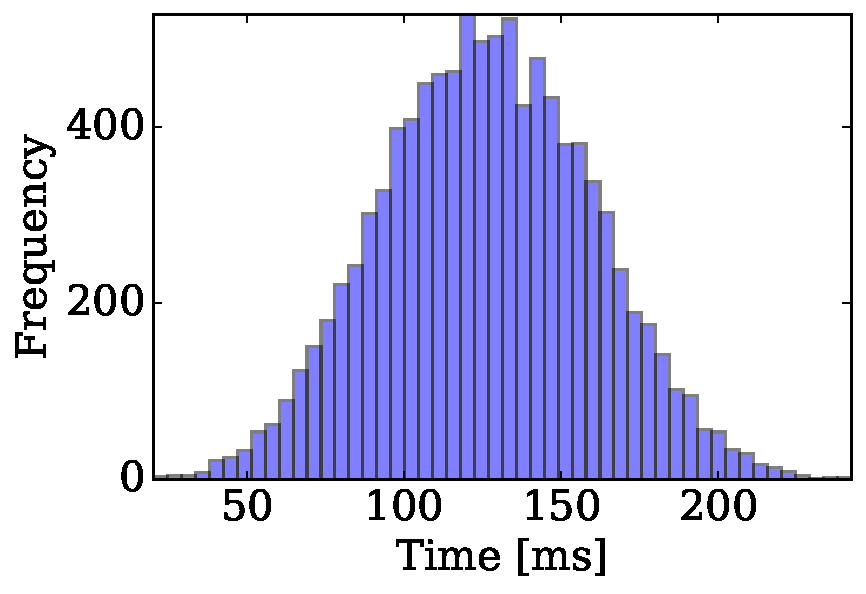
\includegraphics[clip, trim=0.2cm 0.3cm 0.4cm 0.2cm,scale=0.225]{TexImg/SF_query_dij_B25.pdf}\\
(a)
\end{minipage}%
\begin{minipage}[t]{.24\textwidth}
\centering
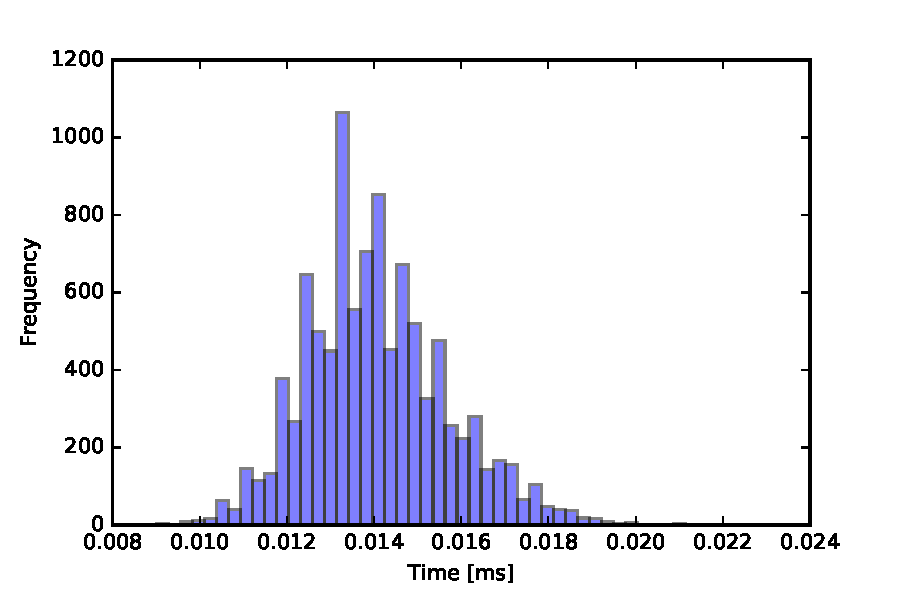
\includegraphics[clip, trim=1.65cm 0.3cm 0.2cm 0.2cm,scale=0.225]{TexImg/SF_query_hl_B25.pdf}\\
(b)
\end{minipage}%
\begin{minipage}[t]{.24\textwidth}
\centering
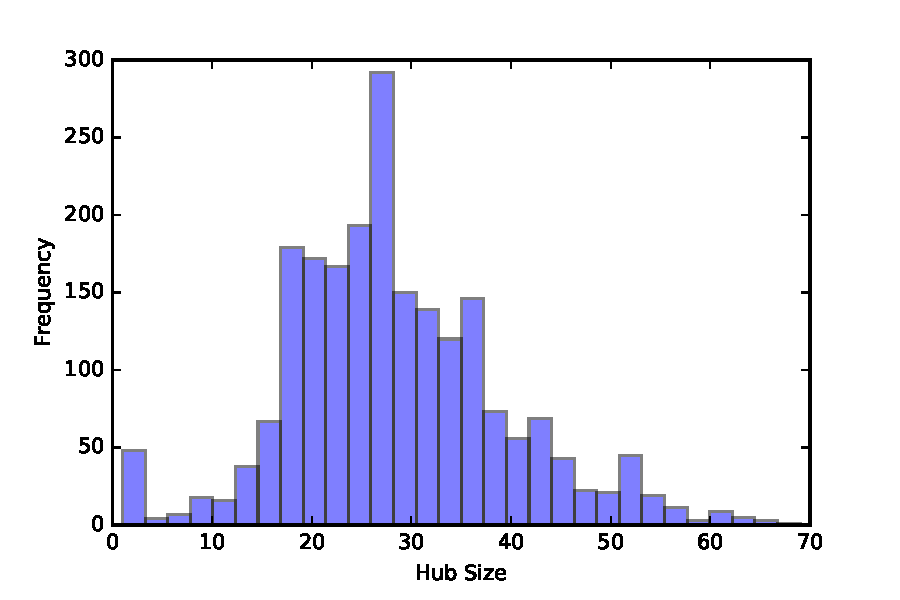
\includegraphics[clip, trim = 1.3cm 0.3cm 0cm 0cm,scale=0.225]{TexImg/SF_bwd_hub_size.pdf}\\
(c)
\end{minipage}%
\begin{minipage}[t]{.24\textwidth}
\centering
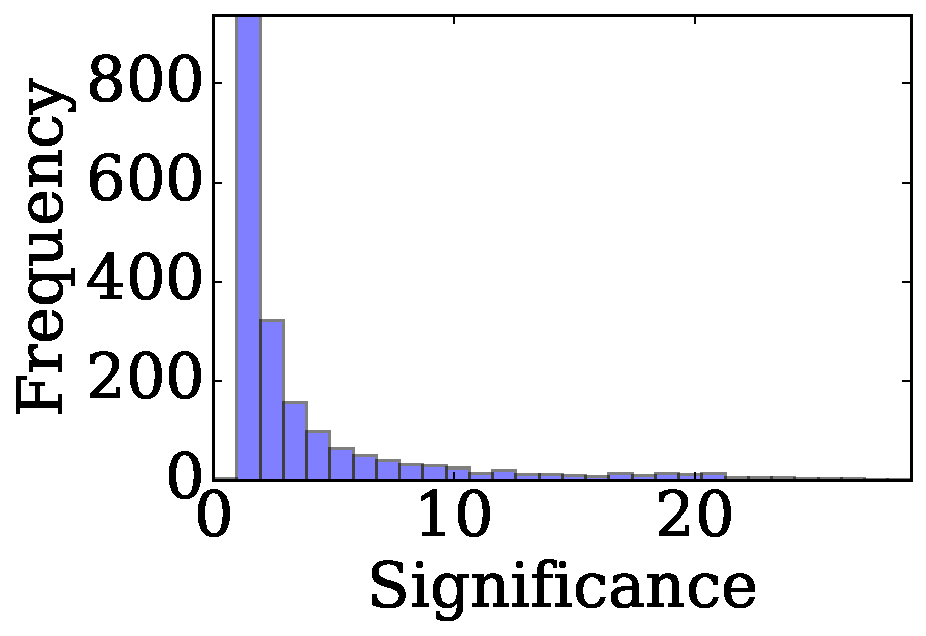
\includegraphics[clip, trim = 1.3cm 0.3cm 0cm 0cm,scale=0.225]{TexImg/significance.pdf}\\
(d)
\end{minipage}
\caption{ Histogram frontier queries for Dijkstra (a) and HL (b). Times are 1000 random pairs in San Francisco augmented with $B=25$.
Size of reverse hubs (c) and significance (d) for frontier queries in San Francisco augmented with $B=25$.
}
\label{fig:SF_query}
\label{fig:SF_bwd_size}
\end{figure}

\subsubsection{Query-time performance}


Table~\ref{tab:performance_results} presents the CSP computation times for different maximum budgets $B$. 
For frontier queries, labelled as `f', the query times are measured as the average of 1000 random $s,t$.
For specific queries, labelled as `s', the times are measured as 1000 random triplets $s,t,b$.
The column for $B=0$ represents the original graph (without augmentation). 
As can be seen in the experimental results, our method finds the constrained shortest path solution on average four orders of magnitude faster than running Dijkstra's algorithm on the augmented graph. 
Preprocessing for frontier queries results in a more compact set of hub labels, since a node $\pp{s,b}$ needs to store information for paths with budget exactly equal to $b$ (in case the path is efficient, otherwise it is not stored).
On the other hand, for specific queries, $\pp{s,b}$ needs to store information for all budgets up to $b$.
The preprocessing time does not include the cover computation, since this is a flat cost of at most the time to preprocess the instance $B=0$.

Note that preprocessing frontier queries in Luxembourg is faster, despite the network being bigger, this can be explained by the structural properties.
For example, in Luxembourg there are more highways and fast roads.

Observe that the \emph{average hub size decreases} in San Francisco for frontier queries, this is because in this instance we use $\Gp$, which prunes away most of the nodes, thus many nodes $\pp{v,b}$ are isolated and have empty hubs.
The longer preprocessing time for frontier queries can be explained as follows.
There are many cases when two nodes are not reachable, to detect this requires Dijkstra to explore the entire graph.
In contrast, for specific queries we add extra edges $\pp{s,b}\pp{s,b-1}$, hence a reachability test ends, in average, earlier.
In the contraction step, we want to remove a node without altering the shortest path, a process that requires many reachability tests.


\subsubsection{Hub sizes and node significance}

We focus the analysis on two meaningful quantities.
The first is hub size, which is well captured by  $\card{\Lb(\pp{t,0})}$ for $t\in V$.
Indeed, for frontier queries the reverse hub is bounding the space requirements; for specific queries the same is true up to a constant factor.
For the second quantity, we define the significance of $s\in V$ as the number of hubs containing $s$, i.e., $\sum_t\sum_b\In{\pp{s,b}\in \Lb(\pp{t,0})}$.
Intuitively, a node is highly significant if belongs to many efficient paths.
Figure~\ref{fig:SF_bwd_size} shows a histogram of these metrics. 

	
\begin{figure}
\begin{minipage}[t]{.53\textwidth}
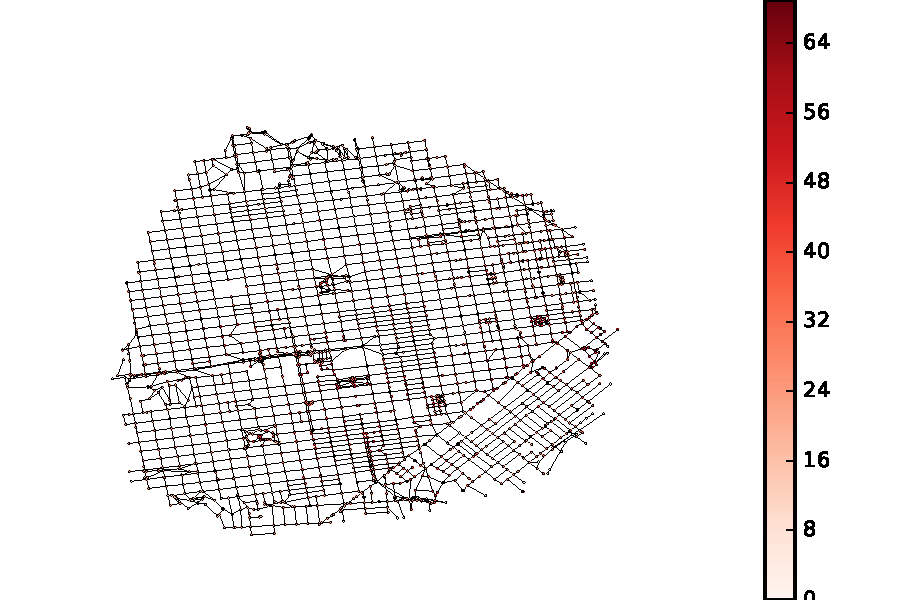
\includegraphics[clip, trim=4.6cm 4.8cm 4.7cm 3cm,height=4.7cm]{TexImg/SF_hub_sizes.pdf}%
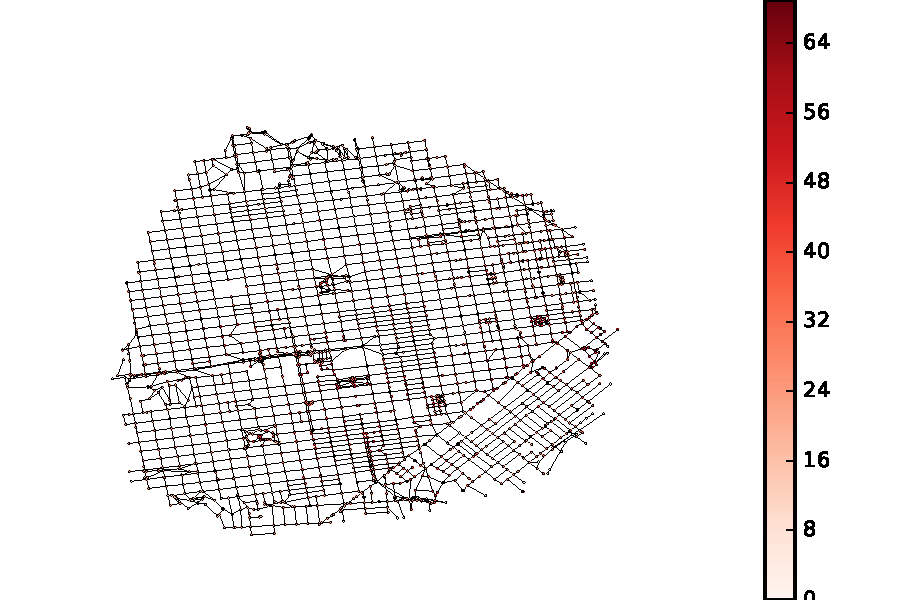
\includegraphics[clip, trim=15.8cm 0cm 0.4cm 1cm,height=4.4cm]{TexImg/SF_hub_sizes.pdf}
\end{minipage}%
\begin{minipage}[t]{.47\textwidth}
\flushright
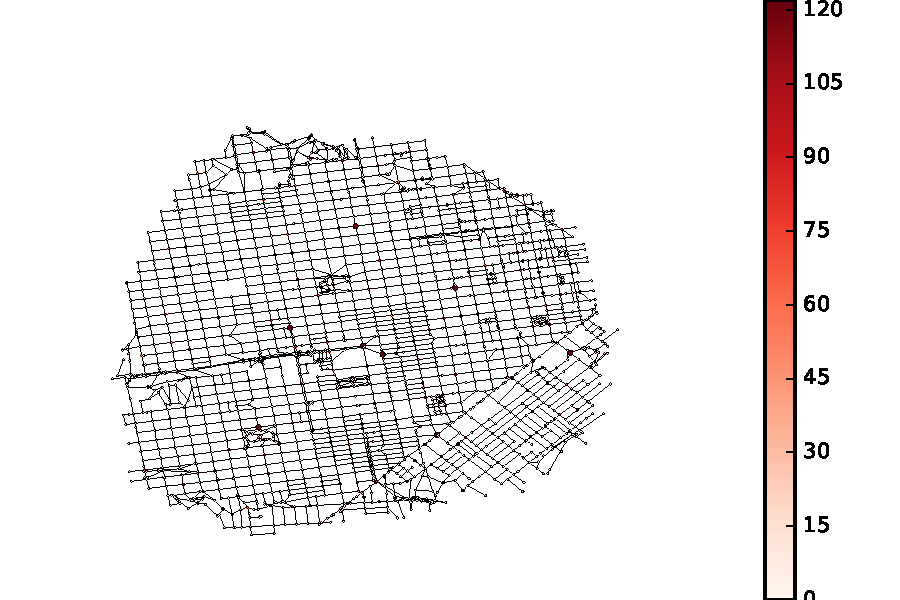
\includegraphics[clip, trim=3.7cm 2.9cm 4.2cm 3cm,height=4.7cm]{TexImg/sig_colapse.pdf}
\end{minipage}
\caption{Heat maps for frontier queries in San Francisco augmented with $B=25$.
On the left we see the hub size. 
Note that the size is not homogeneous, but rather we can observe clusters and neighborhoods tend to be similar.
On the right the significance.
The most significant nodes have been drawn bigger.
The top 3 most significant correspond to Geary Blvd \& Gough St, Franklin St \& O'Farrel St and Market St \& Polk St.
}
\label{fig:heat_maps}
\end{figure}

\cref{fig:heat_maps} presents the spatial relationships between the hub size and significance in the San Francisco network. 
\cref{fig:map_LU} shows the spatial distribution of significance in the Luxembourg network.
We observe that highly significant nodes tend to have small hub size.
The intuition is simple, if most hubs contain $s$, then is easier for $s$ to satisfy the cover property with a small hub.
Note also that the hub size resembles an harmonic function; nodes are mostly similar to their neighbors.

\begin{figure}
\centering
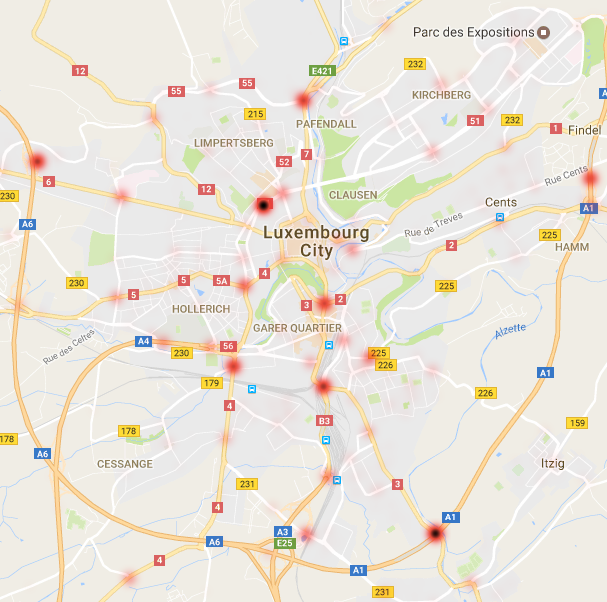
\includegraphics[scale=0.3]{TexImg/map_LU_sig.png}
\caption{Heat map of significance for frontier queries in Luxembourg City augmented with $B=25$.
Notice how the highly significant nodes are in main road crossings.}
\label{fig:map_LU} 
\end{figure}

% ensure same length columns on last page (might need two sub-sequent latex runs)
\balance

%ACKNOWLEDGMENTS are optional
\section{Acknowledgments}

The authors would like to thank Moritz Kobitzsch for sharing sanitized versions of the San Francisco and Luxembourg road networks.

\bibliographystyle{abbrv}
\bibliography{biblio} 


\begin{appendix}

\section{Different notions of HD}
\label{app:generalhd}
% !TEX root = main_vldb.tex
The definition of HD that we use is tailored for HL note, however, that it is the ones used in \cite{highway2013}. 
We now discuss how our results extend to the stronger definition.

The stronger version defines a path $P$ to be $r$-significant if, by adding at most one hop at each end, we get a shortest path $P'$ longer than $r$.
The path $P'$ is called an $r$-witness for $P$.
Intuitively, a path is significant if it represents a long path.
Observe that, if $P\in\PS$ is such that $\ell(P)>r$, then $P$ is $r$-significant by definition.
We remark also that a path can have many $r$-witnesses.

Finally, the path neighborhood must also be strengthened.
The path $P\in\PS$ belongs to $\Sf_r(v)$ if, $P$ has some $r$-witness $P'$ such that $\dist(v,P')\leq 2r$.
The reverse neighborhood $\Sb_r(v)$ is defined analogously.
With this modified versions of $r$-significant and neighborhood, the notions of LSHS and HD are the same as our previous definitions.

Under this stronger notion, we have  $\Delta\leq h$ and $\alpha\leq h+1$.
Additionally, this definition allows proving results for CH.
Finally, we show that under the stronger definition, CHD and HD can still be off by a factor of $n$.

\begin{proposition}\label{prop:treelike}
For any $h$, we can construct a family of networks such that the sparsity of LSHS is $h$ and that of EPHS is arbitrarily worse than $h$.
\end{proposition}
\begin{proof}
First, we construct an example where the sparsity grows from $h$ to $h^2$.
Consider an $h$-ary tree rooted at $u$ with three levels, i.e., with $1+h+h^2$ nodes.
Now add a node $v$ with $h$ children as in Figure~\ref{fig:treelike}. 
The grandchildren of $v$ are the same as the grandchildren of $u$.

All the edges are bidirectional and have unit cost.
The lengths are as follows: $ux_i$ and $vy_i$ (dashed in Figure~\ref{fig:treelike}) are zero; $uv$ and from $y_i$ to the leafs is one; from $x_i$ to the leafs is three.
It is easy to see that the sparsity of a LSHS is $h+1$.

On the other hand, every leaf $w$ is a $2$-efficient path.
Indeed, it can be extended to $x_iw$ that is the shortest path from $x_i$ to $w$ with constraint 1.
All the leafs are in the ball $B_4(u)$, so the sparsity is at least $h^2$.

\begin{figure}
\centering
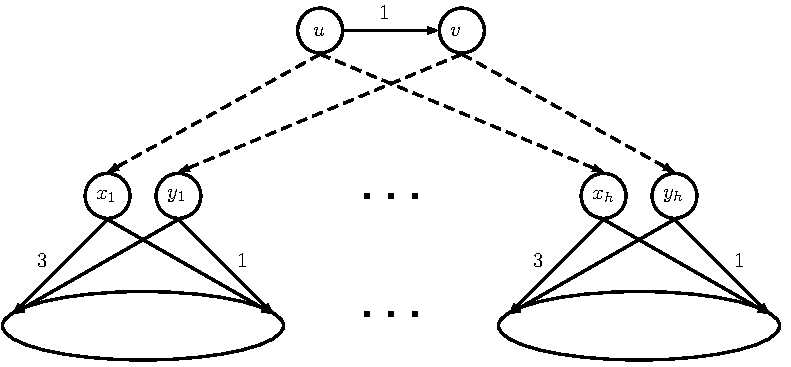
\includegraphics[scale=0.5]{TexImg/Treelike.pdf}
\caption{Example where CHD is much larger than the HD.}\label{fig:treelike}
\end{figure}

The general case works in the same fashion.
We make the sparsity grow to $h^k$ by creating two complete, $k$-level, $h$-ary trees $T$ and $T'$.
Connect the root of $T$ to the root of $T'$ and the leafs of both trees are shared.
Observe that the number of nodes is 
\begin{align*}
n &=[\text{$k$-level $h$-ary tree}] + [\text{$(k-1)$-level $h$-ary tree}]\\
&= ({h^{k+1}-1})/({h-1}) + ({h^k-1})/({h-1}),
\end{align*}
therefore the sparsity is $\Theta(n)$, the worst possible.
\end{proof}

% \section{Contraction Hierarchies}
% \label{sec:ch}
We present here how to extend the concept of HD in order to prove the efficiency of CH in directed graphs.

\begin{definition}
	For $r>0$, the shortest path $P\in\calP$ is $r$-significant if we can add at most one vertex at each end of $P$ to obtain a shortest path $P'\in\calP$ such that $\ell(P')>r$.
	The path $P'$ is called an $r$-witness of $P$.
	We denote $\calP_r$ as the set of all $r$-significant paths.
\end{definition}


Intuitively, a path is significant if it represents a long path.
Observe that, if $P\in \calP$ is such that $\ell(P)>r$, then $P$ is $r$-significant by definition.
We remark also that a path can have many $r$-witnesses.

\begin{definition}
	For $r>0$, an $(h,r)$-LSHS is a set $C\subseteq V$ satisfying: 
	\begin{enumerate}
		\item The set $\calP_r$ is hit by $C$: for every $P\in\calP_r$, $P\cap C\not=\varnothing$.
		\item $C$ is $h$-sparse: for every $v\in V$, $\card{\Bb_{2r}(v)\cap C}\leq h$ and $\card{\Bf_{2r}(v)\cap C}\leq h$.
	\end{enumerate}
\end{definition}

The following is not the usual notion of a sphere.
For $v\in V$, we are interested in paths, not points, close to $v$.
We do not say that $P$ is close to $v$ if $\dist(v,P)$ is small, but rather if $P$ has some $r$-witness $P'$ with $\dist(v,P')$ small.


\begin{definition}
	For $v\in V, r>0$, the path neighbourhood  $\Sf_r(v)$ is defined as the set of paths $P\in\calP_r$ such that $P$ has some $r$-witness $P'$ with $\dist(v,P')\leq 2r$.
	The neighbourhood $\Sb_r(v)$ is defined analogously.
\end{definition}

\begin{definition}
	The network $(G,\ell)$ has HD $h$ if, for every $r>0, v\in V$, there exists $H_{v,r}\subseteq V$ such that $\card{H_{v,r}}\leq h$ and $H_{v,r}$ hits every path in $S_r^+(v)$ and every path in $S_r^-(v)$.
\end{definition}


\subsection{Additional Data Requirements}

Given a rank in the nodes, the shortcut process works as in the non-directed case:
\begin{enumerate}
	\item Let $G'$ be a temporary copy of $G$.
	\item Remove nodes of $G'$ and its edges in increasing rank.
	\item When removing $v$, if some unique shortest path in $G$ uses $uvw$, add $(u,w)$ to $G'$ with length $\ell(u,v)+\ell(v,w)$.
\end{enumerate}

Call $E^+$ the set of edges created in the shortcut process.
A source-destination query runs bidirectional Dijkstra, but each search only considers paths of increasing ranks.

As in the non-directed case, let $Q_i=C_i\setminus \cup_{j>i}C_j$ be the partition of $V$.
All the ranks in $Q_i$ are smaller than those in $Q_{i+1}$, within each $Q_i$ the rank is arbitrary.

\begin{lemma}\label{lemma:intshort}
	Let $P$ be a shortest path in the original graph.
	If $P$ has at least three vertices and $\ell(P)>2^{\gamma}$, then some internal vertex of $P$ belongs to a level $Q_x$, $x>\gamma$.
\end{lemma}
\begin{proof}
	The path $P'$ obtained by removing the endpoints of $P$ is $\ell(P)$-significant.
	By definition of the $C_i$'s, $C_{\gamma+1}$ hits $P'$ at some node $u$.
	By construction of the partition, $u\in Q_x$ with some $x>\gamma$. 
\end{proof}

Now we show that each node adds at most $h$ to its out-degree for each $Q_i$, so the process adds at most $h\log D$ to the out-degree of each node.
\begin{lemma}
	Assume the network admits the $C_i$'s.
	For any $v$ and fixed $j$, the number of shortcuts $(v,w)$ with $w\in Q_j$ is at most $h$.
\end{lemma}
\begin{proof}
	Let $i$ be the level such that $v\in Q_i$ and define $\gamma:=\min(i,j)$.
	We claim that $w\in \Bf_{2^\gamma}(v)$.
	Assume the claim, then the number of shortcuts is at most $\card{Q_j\cap \Bf_{2^\gamma}(v)}$, but using local sparsity and set inclusion:
	\[
	\card{Q_j\cap \Bf_{2^\gamma}(v)}\leq \card{C_j\cap\Bf_{2\cdot 2^{j-1}}(v)} \leq h.
	\]
	
	All that remains is to prove the claim.
	The shortcut $(v,w)$ was created when the process removed the last internal vertex of the shortest path $P(v,w)$ in $G$.
	Necessarily all the internal vertices are in levels at most $\gamma$, because they were removed before $v$ and $w$, hence they have lower rank.
	Finally, apply Lemma~\ref{lemma:intshort} to conclude that $\ell(P(v,w))\leq 2^\gamma$.
\end{proof}

We need to bound the in-degree, because it could be that some node $v$ is receiving many edges.
The proof is basically the same.
\begin{lemma}
	Assume the network admits the $C_i$'s.
	For any $v$ and fixed $j$, the number of shortcuts $(w,v)$ with $w\in Q_j$ is at most $h$.
\end{lemma}
\begin{proof}
	Same as in the previous lemma, but now $w\in \Bb_{2^\gamma}(v)$.
\end{proof}

We can conclude now that the number of shortcuts, i.e.\ $\card{E^+}$, is at most $2nh\log D$.

\subsection{Query Time}

As we mentioned before, the query performs Dijkstra from the source and target, but always constructing paths of increasing rank.
When scanning a vertex $v$, the forward search has a label $\dist(s,v)'$. 
The labels always satisfy $\dist(s,v)'\geq\dist(s,v)$, but, since the algorithm only goes to higher ranks, equality is not guaranteed.

We add a pruning rule analogous to the non-directed case: when the forward search scans a node $v$, if $(v,w)\in E\cup E^+$ and $w\in Q_i$, then $w$ is added to the priority queue only if $\text{rank}(w)>\text{rank}(v)$ and $\dist(s,v)'+\ell(v,w)\leq 2^i$.
For the backward search, the condition is the analogous $\dist(v,t)'+\ell(w,v)\leq 2^i$ when $(w,v)\in  E\cup E^+$.

\begin{proposition}
	The query with additional pruning returns the correct distance.
	Additionally, each Dijkstra scans at most $h$ nodes in each level.
\end{proposition}
\begin{proof}
	Let us analyse the forward search.
	Say the node $v$ is being scanned, $w\in Q_i$ is a candidate and $\dist(s,v)'+\ell(v,w)>2^i$.
	If the current path $P'$ to $w$ is optimal, then $P(s,w)$ is $2^i$-significant and it is hit by $C_{i+1}$. 
	As a consequence, $P(s,w)$ contains an internal vertex with higher rank than $w$.
	This vertex cannot be in $P'$ nor a shortcut containing it, thus contradicting the optimality of $P'$.
	We conclude that $P'$ is not optimal and $w$ can be ignored.
	
	Bounding the number of scanned nodes is easy; every $w\in Q_i$ added to the queue satisfies $w\in \Bf_{2^i}(s)$, so applying local sparsity we finish the proof.
\end{proof}

As a result, the forward search adds at most $h\log D$ nodes to the queue;
each of node amounts to $O(\text{outdeg} (G^+))$ operations, i.e., $O(\text{outdeg}(G) + h\log D)$ operations.


\section{CHD vs. HD: Extensions}
\label{app:extn}

We start by comparing the HD of the union of two systems.
So far we have only used the structure of shortest paths in $G$, which, naturally, does not capture all the information in the network.
It is natural to think that there is structure if we look, for example, only free edges.

Let $G_0$ be obtained from $G$ by removing all the edges with cost.
The networks $G$ and $G_0$ define two hierarchies of roads; shortest paths in $G_0$ are free, but not as fast as the ones in $G$.
Our main hypothesis now is that an efficient path $P$ does not alternate between these two hierarchies.
For example, a path that enters and exits multiple times a highway is not desirable because of turning costs.

\begin{proposition}
Let $\calQ,\calQ'$ be two path systems with HD $h$ and $h'$ respectively.
The HD of the system $\calQ\cup\calQ'$ is at most $h+h'$.
\end{proposition}
\begin{proof}
Given $v\in V$, the union of $H_{v,r}$ and $H_{v,r}'$ hits all the paths in $S_r(v,\calQ)\cup S_r(v,\calQ')$.
\end{proof}

We now relax the assumption that a system witnesses another.
It could be that the efficient paths are sometimes witnessed by free paths and sometimes by shortest paths.

\begin{definition}
We say that $\PE$ does not alternate between $\calQ$ and $\calQ'$ if, for some $\beta,\beta'>0$, each path $P\in\PE$ is either $\beta$-witnessed by some $Q\in\calQ$ or $\beta'$-witnessed by $Q'\in\calQ'$.
\end{definition}

\begin{theorem}
Assume that $G$ has doubling dimension $\alpha$ and $\calQ,\calQ'$ are systems with HD $h,h'$ respectively.
If $\PE$ does not alternate, then it admits $(\alpha^{\log\beta}h+\alpha^{\log\beta'}h',r)$-EPHS.
\end{theorem}


\subsubsection{Correlated Costs}
We have studied so far the case where $c(P)$ is just the sum of individual edge costs.
In practice it could be that the cost depends on combinations of arcs.
Think of a turn in a road network; we can turn right quickly, but turning left means waiting for a green arrow in most cases.
Another example is minimizing expectation subject to bounded variance.
If there is no independence, the variance of a path is not the sum of individual variances.

We explain now how to deal with more general cases using the same framework.
Assume the cost function $c_2:E\times E\to \N\cup \{0\}$ depends on pairs of edges, so if a path is $P=e_0e_1\ldots e_k$, then the cost would be $c_2(P)=\sum_{i=1}^{k}c_2(e_{i-1},e_i)$.
The nodes in the augmented graph will be triplets $\pp{u,v,b}$, where $v$ is the current state, $u$ is the previous state and $b$ is the available budget.
The arcs are given by
\[
(\pp{u,v,b},\pp{v,w,b'}), \quad uv,vw\in E, b'=b-c_2(u,v,2).
\]

Define analogously the concept of efficient paths.
It is easy to see that, as in the previous case, shortest paths in the augmented graph are efficient paths.
The system $\tilde\PE$ of such paths may also allow for a $\beta$-witness.
With the previous properties we can construct the hub labels in the same fashion to prove the following result.

\begin{theorem}
Assume the system $\tilde\PE$ has HD $\tilde h$.
Then, there exists HL such that, queries $s,t,b$ can be answered in time $\Or(b\tilde h\log D)$ and the space requirement is $\Or(Bn\Delta\cdot B\tilde h\log D)$ \todo{double check this}.
In particular, if $\calP$ is a $\beta$-witness for $\tilde \PE$, then $\tilde h\leq h2^{\log_2\beta}$. 
\end{theorem}


 \section{Additional Proofs}
\label{sec:proofs}
% !TEX root = main_vldb.tex

\begin{proof}[of Theorem \ref{thm:markedhubs}]
	To get this stronger bound, we need to modify the HL construction. The algorithm for forward hub construction is given in Algorithm~\ref{alg:forwardhub}, and for reverse hubs in Algorithm~\ref{alg:reversehub}. Note that the two must be run sequentially, as the latter uses the nodes marked in the former.
	
	
	We make the forward hubs $\Lf(\pp{v,b})$ slightly bigger by storing, for each node the distance from $\pp{v,b}$ and also the \emph{budget surplus}.
	Let $C_i$ be the $(h_c,2^{i-1})$-EPHS and $\PE_{s,t}$ the efficient paths from $s$ to $t$.
	
	Observe that, whenever a node $v\in C_i$ is added, $v\in \Bf_{2^i}(s)$ guarantees that at most $h_c$ such points are needed for the whole process.
	Additionally, every such $v$ is added at most $g(b)$ times in the hub of $\pp{s,b}$.
	The data requirement guarantee follows.
	
	The bound for data requirements is $g(B) h_c\log D$, the argument is analogous to the forward case.
	Finally, we need to prove the cover property.
	Take any query $SP(\pp{s,b},t^-)$ and let $P$ be the solution.
	In $Lf(\pp{s,b})$ there is a node $v_P$ added by Algorithm~\ref{alg:forwardhub}.
	By construction, the same node $v_P$ was added to $\Lb(\pp{d,0})$. The result follows.
\end{proof}

\begin{algorithm}[!ht]
	\small
	\caption{Construction of forward hub}
	\label{alg:forwardhub}
	\begin{algorithmic}[1]
		\Require Node $s\in V$, efficient paths $\PE_{s,t}\,\forall\,t$, EPHS $\crl*{C_i}$.
		\Ensure Forward hubs $Lf(\pp{s,b})$ for $b=0,\ldots,B$ and a marked node $v_P$ for every path.
		\State Order each $\PE_{s,t}$ by increasing cost and remove paths consuming more than $B$.
		\For{$t\in V\setminus s$}
		\For{$P\in\Pst^E$}
		\State $b\gets c(P)$, $b'\gets c(P')$, where $P'$ is the next path in the list ($b'=B$ if no such path).
		\State Find the largest $i$ such that $P$ is $2^{i-1}$-efficient.
		\State Find $v\in C_i$ hitting $P$ and mark $v$ as $v_P$.
		\State Add $\pp{v,c(P[v,t])}$ to $L(\pp{s,b})^+$  with distance $\ell(P[s,v])$ and surplus zero.
		\For{$x$ between $b$ and $b'$}
		\State Add $\pp{v,c(P[v,t])}$ to $L(\pp{s,x})^+$  with distance $\ell(P[s,v])$ and surplus $x-b$.
		\EndFor
		\EndFor
		\EndFor
	\end{algorithmic}
\end{algorithm}

\begin{algorithm}[h]
	\small
	\caption{Construction of reverse hub}
	\label{alg:reversehub}
	\begin{algorithmic}[1]
		\Require Node $t\in V$, efficient paths $\Pst^E\,\forall\,s$, marked nodes and EPHS $C_i$.
		\Ensure Backward hub $\Lb(\pp{t,0})$.
		\State Order each $\Pst^E$ by increasing cost and remove paths consuming more than $B$.
		\State $\Lb(\pp{t,0})\gets \varnothing$
		\For{$s\in V\setminus t$}
		\For{$P\in\Pst^E$}
		\State Find the largest $i$ such that $P$ is $2^{i-1}$-efficient.
		\State Take $v$ as the marked node $v_P$.
		\State Add $\pp{v,c(P[v,t])}$ to $\Lb(\pp{t,0})$ with distance $\ell(P[v,t])$.
		\EndFor
		\EndFor
	\end{algorithmic}
\end{algorithm}


\begin{proof}[of Proposition~\ref{prop:poly_lshs}]
Denote $S_r(v):=\Sf_r(v,\calQ)\cup\Sb_r(v,\calQ)$. 
Observe that, for fixed $v\in V$, the set system $(E,\{\pi(Q):Q \in S_r(v)\})$ admits a hitting set of size $h\Delta$.
Indeed, we know that exists $H_{v,r}\subseteq V$, $\card{H_{v,r}}\leq h$, hitting every path in $\Sf_r(v,\calQ)$ and in $\Sb_r(v,\calQ)$.
The desired hitting set consists of all the edges adjacent to a node in $H_{v,r}$.

If the minimum size of a set system is $s$ and the VC-dimension is $d$, then the algorithm in \cite{vc_dim_hitting} obtains, in polynomial time, a hitting set of size at most $\Or(sd\log(sd))$.
In particular, we can use the algorithm to obtain a set $\tilde F_{v,r}\subseteq E$, of size at most $h'=\Or(h\Delta\log(h\Delta))$, hitting the set system $(E,\{\pi(Q):Q \in S_r(v)\})$ .

Consider the set $F_{v,r}\subseteq V$ that contains all the endpoints of edges in $\tilde F_{v,r}$.
It follows that $F_{v,r}\subseteq V$ can be obtained in polynomial time and is a hitting set for $S_r(v)$ of size $\card{F_{v,r}}\leq 2h'$.
Assume for now that we know the value of $h$.
Note that the value $h'$ can be computed from $h$ and the guarantee given by the oracle, i.e., the constant inside the big-O.
We construct the $(2h',r)$-LSHS iteratively.
At each iteration $i$ we maintain the following invariant: $C_i$ hits every path in $\calQ_r$.
In an iteration we check if $C_i$ is locally sparse, if not, we strictly reduce the cardinality of $C_i$ while maintaining the invariant.
Start with $C_0=V$. 
Let $B_{2r}(v):=\Bf_{2r}(v)\cup \Bb_{2r}(v)$.
Assume $v\in V$ is such that $\card{B_{2r}(v)\cap C_i}>2h'$ and let $C_{i+1}:=(C_i\setminus B_{2r}(v))\cup F_{v,r} $.
The cardinality strictly decreases and we only need to check the invariant.
Consider the paths hit by nodes removed in $C_i$, this set is
\begin{align*}
&\hspace{-1cm}\{Q\in\calQ_r: Q\cap C_i\cap B_{2r}(v)\neq \varnothing\}\\
&\subseteq \{Q\in\calQ_r: Q\cap B_{2r}(v)\neq \varnothing\} \subseteq S_r(v).
\end{align*}
Since $F_{v,r}$ hits $S_r(v)$, the proof is completed.

If we do not know the value of $h$, we can do a doubling search for $h'$. 
Indeed, if the guess of $h'$ is low, then at some point it could be that $\card{F_{v,r}}>2h'$, then we double $h'$ and restart the process.
\end{proof}




\end{appendix}

\end{document}